% Wysp: architecture (English edition)
% Build: cd docs/architecture && xelatex wysp-architecture.tex && xelatex wysp-architecture.tex
% The French pre-implementation design document is kept in fr/.
\documentclass[11pt,a4paper]{article}

\usepackage{fontspec}
\usepackage[english]{babel}
\setmainfont{texgyrepagella}[Extension=.otf, UprightFont=*-regular, BoldFont=*-bold, ItalicFont=*-italic, BoldItalicFont=*-bolditalic]
\setsansfont{texgyreheros}[Extension=.otf, UprightFont=*-regular, BoldFont=*-bold, ItalicFont=*-italic, BoldItalicFont=*-bolditalic]
\setmonofont{texgyrecursor}[Extension=.otf, UprightFont=*-regular, BoldFont=*-bold, ItalicFont=*-italic, BoldItalicFont=*-bolditalic, Scale=0.88]

\usepackage[margin=2.0cm,headheight=14pt]{geometry}
\usepackage{xcolor}
\usepackage{graphicx}
\usepackage{tikz}
\usetikzlibrary{arrows.meta,positioning,shapes.geometric,fit,backgrounds,calc}
\usepackage{booktabs,array,multirow,xltabular}
\usepackage{enumitem}
\usepackage{listings}
\usepackage[most]{tcolorbox}
\usepackage{fancyhdr}
\usepackage{titlesec}
\usepackage{url}
\usepackage{multicol}
\usepackage{float}
\usepackage[hidelinks]{hyperref}
\usepackage[nameinlink,noabbrev]{cleveref}

% ------------------------------------------------------------------ brand colours
\definecolor{night}{HTML}{120532}
\definecolor{surface}{HTML}{1D0E4A}
\definecolor{lilac}{HTML}{CA84FC}
\definecolor{pink}{HTML}{FE7C9C}
\definecolor{lavender}{HTML}{F4E5FD}
\definecolor{violet}{HTML}{6503FC}
% print-friendly variants
\definecolor{inkpurple}{HTML}{3B2A80}
\definecolor{lilacdeep}{HTML}{8A3FD1}
\definecolor{pinkdeep}{HTML}{D6385F}
\definecolor{muted}{HTML}{6B5B95}
\definecolor{okgreen}{HTML}{15803D}
\definecolor{codebg}{HTML}{FAF6FE}

% ------------------------------------------------------------------ layout
\titleformat{\section}{\Large\sffamily\bfseries\color{night}}{\thesection}{0.8em}{}
\titleformat{\subsection}{\large\sffamily\bfseries\color{inkpurple}}{\thesubsection}{0.7em}{}
\titleformat{\subsubsection}{\normalsize\sffamily\bfseries\color{inkpurple}}{\thesubsubsection}{0.6em}{}
\titlespacing*{\section}{0pt}{14pt}{6pt}
\pagestyle{fancy}
\fancyhf{}
\fancyhead[L]{\sffamily\small\color{muted} Wysp \textbullet{} Architecture}
\fancyhead[R]{\sffamily\small\color{muted} Contract 1.1.0 \textbullet{} November 2026}
\fancyfoot[C]{\sffamily\small\thepage}
\renewcommand{\headrulewidth}{0.3pt}
\setlist{itemsep=2pt,topsep=4pt}
\setlength{\parskip}{4pt}
\setlength{\parindent}{0pt}
\setlength{\emergencystretch}{3em}
\renewcommand{\arraystretch}{1.15}
\hypersetup{colorlinks=true,linkcolor=lilacdeep,urlcolor=lilacdeep,citecolor=lilacdeep}

% ------------------------------------------------------------------ code
\lstdefinestyle{wysp}{
  basicstyle=\ttfamily\footnotesize, backgroundcolor=\color{codebg}, frame=single, rulecolor=\color{lilac!60},
  breaklines=true, columns=fullflexible, keepspaces=true, showstringspaces=false,
  xleftmargin=2pt, xrightmargin=2pt, aboveskip=6pt, belowskip=6pt}
\lstset{style=wysp}

% ------------------------------------------------------------------ boxes
\newtcolorbox{keybox}[1][]{enhanced, colback=lilac!14, colframe=lilacdeep, boxrule=0.6pt, arc=2mm,
  left=6pt, right=6pt, top=4pt, bottom=4pt, fonttitle=\sffamily\bfseries, title={#1}}
\newtcolorbox{wherebox}{enhanced, colback=codebg, colframe=lilac!70, boxrule=0.5pt, arc=2mm,
  left=6pt, right=6pt, top=3pt, bottom=3pt, before skip=10pt, after skip=6pt, before upper={\raggedright\small}, before upper={\raggedright\small},
  fonttitle=\sffamily\bfseries\small, title={Where to look in the repository}}
\newtcolorbox{notebox}{enhanced, colback=pink!10, colframe=pinkdeep!70, boxrule=0.5pt, arc=2mm,
  left=6pt, right=6pt, top=3pt, bottom=3pt}

% ------------------------------------------------------------------ macros
\newcommand{\code}[1]{\texttt{#1}}
\newcommand{\file}[1]{\texttt{\small #1}}
\newcommand{\pobs}{\textsf{observed}}
\newcommand{\pinf}{\textsf{inferred}}
\newcommand{\pill}{\textsf{illustrative}}
\newcolumntype{L}[1]{>{\raggedright\arraybackslash}p{#1}}
\newcolumntype{Y}{>{\raggedright\arraybackslash}X}
\renewcommand{\UrlFont}{\ttfamily\small}

% ------------------------------------------------------------------ TikZ styles
\tikzset{
  fig/.style={font=\sffamily\scriptsize, align=center},
  node distance=6mm,
  mod/.style={draw=lilacdeep, fill=white, rounded corners=1.5pt, align=center, minimum height=0.6cm, inner sep=2.5pt},
  zone/.style={draw=#1, fill=#1!6, rounded corners=3pt, inner sep=6pt},
  arr/.style={-{Stealth[length=2mm]}, thick, color=inkpurple},
  biarr/.style={{Stealth[length=2mm]}-{Stealth[length=2mm]}, thick, color=inkpurple},
  linkdash/.style={dashed, thick, color=muted},
  lab/.style={font=\sffamily\tiny\itshape, text=muted, inner sep=1pt},
}

% Sequence diagrams: \actor{name}{x}{label}, \msg{from}{to}{y}{text}, \note{actor}{y}{text}
\newcommand{\seqlife}{5.0}
\newcommand{\actor}[3]{%
  \node[draw=lilacdeep, fill=lilac!20, rounded corners=2pt, minimum width=1.7cm, minimum height=0.55cm, inner sep=2pt, align=center, font=\sffamily\scriptsize\bfseries] (#1) at (#2,0) {#3};
  \draw[color=muted, dashed] (#1.south) -- ++(0,-\seqlife);}
\newcommand{\msg}[4]{%
  \draw[-{Stealth[length=2mm]}, thick, color=inkpurple] ($(#1.south)+(0,-#3)$) -- node[above, fill=white, font=\sffamily\tiny, text=night, inner sep=1pt, align=center] {#4} ($(#2.south)+(0,-#3)$);}
\newcommand{\ret}[4]{%
  \draw[-{Stealth[length=2mm]}, thick, dashed, color=inkpurple] ($(#1.south)+(0,-#3)$) -- node[above, fill=white, font=\sffamily\tiny, text=night, inner sep=1pt, align=center] {#4} ($(#2.south)+(0,-#3)$);}
\newcommand{\note}[3]{%
  \node[draw=pinkdeep!70, fill=pink!15, font=\sffamily\tiny, inner sep=2pt, align=center, rounded corners=1pt] at ($(#1.south)+(0,-#2)$) {#3};}

\begin{document}
\fontsize{10.2}{12.6}\selectfont

% ------------------------------------------------------------------ title page
\begin{titlepage}
\begin{tikzpicture}[remember picture,overlay]
  \fill[night] (current page.north west) rectangle ([yshift=-11cm]current page.north east);
  \foreach \x/\y/\r/\o in {16.5/-2.0/0.45/0.5, 17.6/-3.1/0.2/0.4, 15.4/-3.4/0.12/0.4}
    \shade[inner color=lilac!80!white, outer color=night, opacity=\o] ([xshift=\x cm, yshift=\y cm]current page.north west) circle (\r cm);
  \node[anchor=west] at ([xshift=2.0cm,yshift=-4.6cm]current page.north west) {
\includegraphics[height=3.4cm]{../brand/mark-color-256.png}};
  \node[anchor=west, text=lavender, font=\sffamily\bfseries\fontsize{50}{56}\selectfont] at ([xshift=6.2cm,yshift=-3.9cm]current page.north west) {Wysp};
  \node[anchor=west, text=lilac, font=\sffamily\Large] at ([xshift=6.25cm,yshift=-5.3cm]current page.north west) {A skeleton for AI tutors of software applications};
  \node[anchor=west, text=lavender!80, font=\sffamily\normalsize] at ([xshift=2.05cm,yshift=-8.4cm]current page.north west) {Kiroween 2026 \textbullet{} Skeleton Crew};
\end{tikzpicture}

\vspace*{10.6cm}
{\sffamily\huge\bfseries\color{night} Architecture\par}
\vspace{0.2cm}
{\sffamily\large\color{inkpurple} How one Core, one Panel and one protocol serve many applications\par}
\vspace{0.9cm}

{\small
\begin{tabularx}{\textwidth}{@{}L{3.4cm}Y@{}}
\textbf{Edition} & English, November 2026. The French design document written before the implementation is kept in \file{docs/architecture/fr/}. \\
\textbf{Describes} & Wysp Core, adapter contract 1.1.0, the Blender, IntelliJ IDEA and Chrome tutors \\
\textbf{Source code} & \url{https://github.com/MELAS-exe/Kiro-Wysp} \\
\textbf{Reading time} & 15 to 20 minutes. Chapters 1 and 2 are enough to understand the idea. \\
\end{tabularx}}

\vfill
\begin{notebox}
\small Every technical statement in this document was checked against the repository at the time of writing. Each chapter ends with a box that names the files to open. The normative specifications are in \file{.kiro/specs/}. The contract itself is the Pydantic models in \file{core/src/wysp\_core/contract/} and the JSON Schemas generated from them in \file{schemas/}.
\end{notebox}
\end{titlepage}

{\small\setlength{\columnsep}{1.2cm}\begin{multicols}{2}\tableofcontents\end{multicols}}
\clearpage

\section{Summary}\label{sec:summary}

\textbf{Wysp is an open-source skeleton for building AI tutors for software applications.} A Wysp tutor reads the real state of an application, explains what it sees, shows the explanation on an interactive board, guides the user through actions with their permission, and checks in the application that the user did what was asked. It speaks, it listens, and it needs one adapter per application.



\begin{figure}[H]
\centering
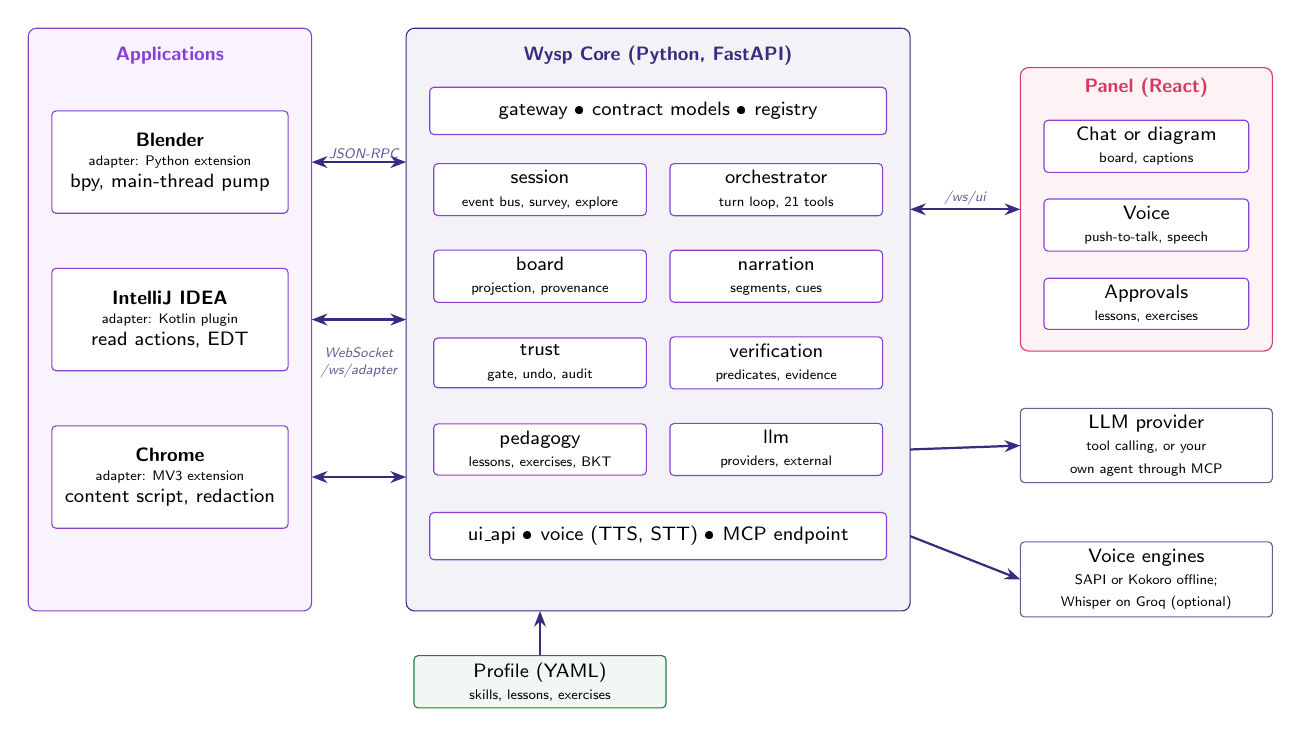
\begin{tikzpicture}[fig, x=1cm, y=1cm]
  % applications and adapters
  \node[zone=lilacdeep, minimum width=3.6cm, minimum height=7.4cm] (apps) at (-6.2,0) {};
  \node[font=\sffamily\bfseries\scriptsize, text=lilacdeep] at (-6.2,3.35) {Applications};
  \foreach \y/\app/\ad in {2.0/Blender/{Python extension\\bpy, main-thread pump}, 0.0/IntelliJ IDEA/{Kotlin plugin\\read actions, EDT}, -2.0/Chrome/{MV3 extension\\content script, redaction}} {
    \node[mod, minimum width=3.0cm, minimum height=1.3cm, align=center] at (-6.2,\y) {\textbf{\app}\\[-1pt]\tiny adapter: \ad};
  }
  % core
  \node[zone=inkpurple, minimum width=6.4cm, minimum height=7.4cm] (core) at (0,0) {};
  \node[font=\sffamily\bfseries\scriptsize, text=inkpurple] at (0,3.35) {Wysp Core (Python, FastAPI)};
  \node[mod, minimum width=5.8cm] (gw) at (0,2.65) {gateway \textbullet{} contract models \textbullet{} registry};
  \node[mod, minimum width=2.7cm] at (-1.5,1.65) {session\\\tiny event bus, survey, explore};
  \node[mod, minimum width=2.7cm] at (1.5,1.65) {orchestrator\\\tiny turn loop, 21 tools};
  \node[mod, minimum width=2.7cm] at (-1.5,0.55) {board\\\tiny projection, provenance};
  \node[mod, minimum width=2.7cm] at (1.5,0.55) {narration\\\tiny segments, cues};
  \node[mod, minimum width=2.7cm] at (-1.5,-0.55) {trust\\\tiny gate, undo, audit};
  \node[mod, minimum width=2.7cm] at (1.5,-0.55) {verification\\\tiny predicates, evidence};
  \node[mod, minimum width=2.7cm] at (-1.5,-1.65) {pedagogy\\\tiny lessons, exercises, BKT};
  \node[mod, minimum width=2.7cm] at (1.5,-1.65) {llm\\\tiny providers, external};
  \node[mod, minimum width=5.8cm] (uiapi) at (0,-2.75) {ui\_api \textbullet{} voice (TTS, STT) \textbullet{} MCP endpoint};
  % panel
  \node[zone=pinkdeep, minimum width=3.2cm, minimum height=3.6cm] (panel) at (6.2,1.4) {};
  \node[font=\sffamily\bfseries\scriptsize, text=pinkdeep] at (6.2,2.95) {Panel (React)};
  \node[mod, minimum width=2.6cm] at (6.2,2.2) {Chat or diagram\\\tiny board, captions};
  \node[mod, minimum width=2.6cm] at (6.2,1.2) {Voice\\\tiny push-to-talk, speech};
  \node[mod, minimum width=2.6cm] at (6.2,0.2) {Approvals\\\tiny lessons, exercises};
  % outside
  \node[mod, minimum width=3.2cm, draw=muted] (llm) at (6.2,-1.6) {LLM provider\\\tiny tool calling, or your\\\tiny own agent through MCP};
  \node[mod, minimum width=3.2cm, draw=okgreen, fill=okgreen!6] (prof) at (-1.5,-4.6) {Profile (YAML)\\\tiny skills, lessons, exercises};
  \node[mod, minimum width=3.2cm, draw=muted] (vox) at (6.2,-3.3) {Voice engines\\\tiny SAPI or Kokoro offline;\\\tiny Whisper on Groq (optional)};
  % arrows
  \draw[biarr] (-4.4,2.0) -- node[lab, above, pos=0.55] {JSON-RPC} (-3.2,2.0);
  \draw[biarr] (-4.4,0.0) -- (-3.2,0.0);
  \draw[biarr] (-4.4,-2.0) -- (-3.2,-2.0);
  \node[lab, align=center] at (-3.8,-0.55) {WebSocket\\{/ws/adapter}};
  \draw[biarr] (3.2,1.4) -- node[lab, above] {/ws/ui} (4.6,1.4);
  \draw[arr] (3.2,-1.65) -- (4.6,-1.6);
  \draw[arr] (3.2,-2.75) -- (4.6,-3.3);
  \draw[arr] (prof.north) -- (-1.5,-3.7);
\end{tikzpicture}
\caption{The whole system. Solid frames are code that is shared by every tutor (Core, Panel). The application, its adapter and its profile are the only parts that change from one tutor to the next. Everything runs on the user's machine; only the LLM provider and the optional cloud speech recognition are remote.}\label{fig:system}
\end{figure}

\subsection*{The skeleton claim}

Everything that is not specific to one application is written once:

\begin{itemize}[leftmargin=1.2em]
  \item \textbf{One Core} (Python). It runs the conversation, the board, the voice, the permission gate, the verification and the learner model. It contains no application vocabulary. A script checks this on every change.
  \item \textbf{One Panel} (React). The same user interface serves every tutor.
  \item \textbf{One protocol} (the adapter contract, version 1.1.0): JSON-RPC 2.0 over WebSocket, defined once as Pydantic models and exported as JSON Schema and TypeScript types.
\end{itemize}

Teaching a new application takes two things and no change to the Core or the Panel: an \textbf{adapter} (code that lets the Core see the application and run a closed list of actions) and a \textbf{profile} (YAML with skills, concepts, lessons and exercises). The repository proves the claim with three tutors:

\begin{center}
\small
\begin{tabularx}{\textwidth}{@{}L{2.9cm}L{2.5cm}Y@{}}
\toprule
\textbf{Tutor} & \textbf{Integration} & \textbf{What it teaches, and how it connects} \\
\midrule
Blender (5.2 LTS) & native & The scene, objects and the modifier stack. A Python extension that runs inside Blender (\code{bpy}). \\
IntelliJ IDEA (2026.2) & native & The student's own project: structure, symbols, problems, refactorings. A Kotlin plugin built on the IntelliJ Platform. \\
Chrome (optional extra) & interface & Web applications, shown through an accessibility-style snapshot of the page. A Manifest V3 extension. \\
\bottomrule
\end{tabularx}
\end{center}

\subsection*{The product promise}

\begin{keybox}[See the context, understand the concept, try the action, verify the result.]
Wysp starts from what is really on the screen (an \emph{observation}), explains one concept in short spoken segments tied to something visible, lets the user try (preferably the user acts, Wysp watches; Wysp acts only when asked and permitted), and verifies the outcome with a predicate evaluated on a fresh observation. The user's autonomy is the goal: the default mode is \emph{guide}, not \emph{do}.
\end{keybox}

Two rules make this trustworthy. Every fact carries a \emph{provenance} (\pobs, \pinf{} or \pill), and nothing is shown as observed unless it came from an adapter. The language model can only \emph{propose} actions: a permission gate decides, the adapter executes, and the Core verifies and undoes the action if the result is wrong.

\subsection*{What a session looks like}

The user opens the Panel next to the application. Wysp surveys the application (counts, structure, available actions) before the first answer. The user asks a question, by typing or by holding Space. Wysp looks at the application, says two or three short sentences, builds the board from real entities, and points at the relevant control inside the application. If a change is useful, Wysp either walks the user through it (guide) or asks for approval and does it (do), then shows the evidence that the change took effect.

\begin{wherebox}
\file{README.md} (run it in two minutes with a mock application, no account needed), \file{core/} (the Core), \file{panel/}, \file{apps/blender-tutor/}, \file{apps/intellij-tutor/}, \file{apps/web-tutor/}, \file{.kiro/specs/} (normative specs).
\end{wherebox}





\section{Concepts and vocabulary}\label{sec:concepts}

The same eleven terms are used in the code, the specs and this document.

\begin{xltabular}{\textwidth}{@{}L{2.6cm}Y@{}}
\toprule
\textbf{Term} & \textbf{Meaning} \\
\midrule
\textbf{Core} & The shared Python engine (package \code{wysp\_core}). It orchestrates the conversation with the language model, builds the board, narrates, enforces permissions, verifies results and tracks what the learner has mastered. It knows no application. \\
\textbf{Adapter} & The application-specific component that implements the adapter contract: \code{observe}, \code{get\_context}, \code{get\_actions}, \code{execute}, \code{undo}, \code{highlight} and events. It lives inside the application (an extension or plugin) and connects to the Core as a WebSocket client. \\
\textbf{Profile} & Application-specific \emph{data} in YAML: skills, a glossary of concepts, lessons and exercises, and a short description of the application for the language model. \\
\textbf{Tutor} & One adapter plus one profile, plugged into the Core. There is one folder per tutor under \file{apps/}. \\
\textbf{Panel} & The single React user interface, shared by all tutors. It shows a chat or a diagram, plays captions and speech, and asks for permissions. It contains no tutoring logic. \\
\textbf{Board} & The visual model of the explanation: nodes, edges, numbered steps and annotations, with a layout (stack, tree, graph or sequence). The Core owns it and sends patches to the Panel. At most 60 nodes. \\
\textbf{Provenance} & The epistemic status of every displayed or spoken fact. \pobs: it comes from an adapter observation of this session. \pinf: the model deduced it. \pill: a teaching example, not the user's state. \\
\textbf{Integration level} & How the adapter sees the application. \code{native}: through its own API. \code{interface}: through the DOM or the accessibility tree. \code{visual}: through screenshots (observations then carry a confidence below 1, and irreversible actions are forbidden). \\
\textbf{Permission gate} & The Core component that decides whether a proposed action may run, and asks the user when policy requires it. The language model cannot bypass it: it has no tool that executes anything. \\
\textbf{Evidence} & The record that proves a verification: the predicate, the actual value, the expected value, the observation id and a timestamp. Its type is \code{verified}, \code{answered} or \code{declared}. \\
\textbf{Mastery} & The learner model's estimate, between 0 and 1, that the learner has acquired a skill. It is updated from evidence with a simplified Bayesian Knowledge Tracing model, and a skill counts as acquired at 0.85. \\
\bottomrule
\end{xltabular}

\subsection{Other words you will meet}

\begin{xltabular}{\textwidth}{@{}L{2.6cm}Y@{}}
\toprule
\textbf{Term} & \textbf{Meaning} \\
\midrule
Observation & A snapshot of the application as a graph of \emph{entities} (each with a stable \code{ref}, a \code{kind}, a label and properties) and \emph{links}. \\
Ref & A stable URI-like identifier of an entity, with one scheme per adapter: \code{blender://object/Candle}, \code{intellij://file/src/Main.java}, \code{web://localhost:5180/page}. \\
Action & A named operation the adapter can perform, declared in a closed catalog with a parameter schema, a risk level and postconditions. \\
Guide and do & Two modes of a proposed action. \emph{Guide}: the user performs it, Wysp watches and verifies. \emph{Do}: Wysp performs it after approval and then verifies. \\
Predicate & A small declarative test (JMESPath comparisons combined with \code{all}, \code{any}, \code{not}) evaluated by the Core on a fresh observation. \\
Survey & The summary of the application the Core collects when an adapter becomes active, so that the first answer is grounded. \\
External mode & The Core runs without a model of its own and the user's own AI agent does the thinking through MCP (\cref{sec:core-llm}). \\
\bottomrule
\end{xltabular}

\subsection{Three principles that shape everything}

\begin{enumerate}[leftmargin=1.4em]
  \item \textbf{The Core knows no application.} No host import (\code{bpy}, browser APIs, IDE APIs) and no application word in \file{core/}. Application knowledge is data (a profile) or code in an adapter. The Core prompts are generic and receive the application description from the manifest and the profile.
  \item \textbf{The model decides what to say and show. The Core decides what is true and what is allowed.} The model chooses which real entities to put on the board but never writes an \pobs{} node itself. It can propose actions but never run them.
  \item \textbf{Local first.} The Core listens on \code{127.0.0.1}, adapters authenticate with a pairing token, browsers are checked against an Origin allowlist, and secrets stay in environment variables.
\end{enumerate}

\begin{wherebox}
\file{.kiro/steering/product.md} (vocabulary and product promise), \file{.kiro/steering/structure.md} (boundary rules), \file{scripts/kiro/hook.py} (the boundary check, run with \code{uv run --no-project python scripts/kiro/hook.py boundaries}).
\end{wherebox}


\section{Architecture}\label{sec:architecture}

\subsection{Components}

Wysp runs entirely on the user's machine. One Python process, the Core, serves the Panel and accepts adapter connections. Each adapter lives inside its host application and dials out to the Core. Figure~\ref{fig:system} shows the parts; this table says what each one is.

\begin{xltabular}{\textwidth}{@{}L{3.0cm}L{2.5cm}Y@{}}
\toprule
\textbf{Component} & \textbf{Language} & \textbf{Role} \\
\midrule
Contract & Python (Pydantic) & Models of every message, JSON Schema export, predicate language, state digest. Single source of truth for the SDKs and the test kit. \\
Wysp Core & Python 3.13 & Gateway, session, orchestrator, board, narration, trust, verification, pedagogy, LLM providers, voice, MCP endpoint. FastAPI and uvicorn. \\
Panel & TypeScript, React 19 & A minimal shell: chat or diagram, captions, voice, permission dialog, lesson and exercise cards. Board drawn with React Flow and ELK layouts, state in Zustand. \\
Adapter SDKs & Python, TypeScript & WebSocket client, action registry with parameter validation, origin tagging, main-thread dispatcher (Python). \\
Contract Test Kit & Python & Plays the Core's part against any adapter and checks the contract. Includes a mock Kanban adapter. \\
Tutors & Python, Kotlin, TypeScript & Blender extension, IntelliJ plugin, Chrome extension, each with its profile. \\
\bottomrule
\end{xltabular}

\subsection{Trust boundaries}

Wysp has one rule for crossing a boundary: data from the other side is data, never an instruction. Figure~\ref{fig:boundaries} shows the zones and what protects each channel.

\begin{figure}[H]
\centering
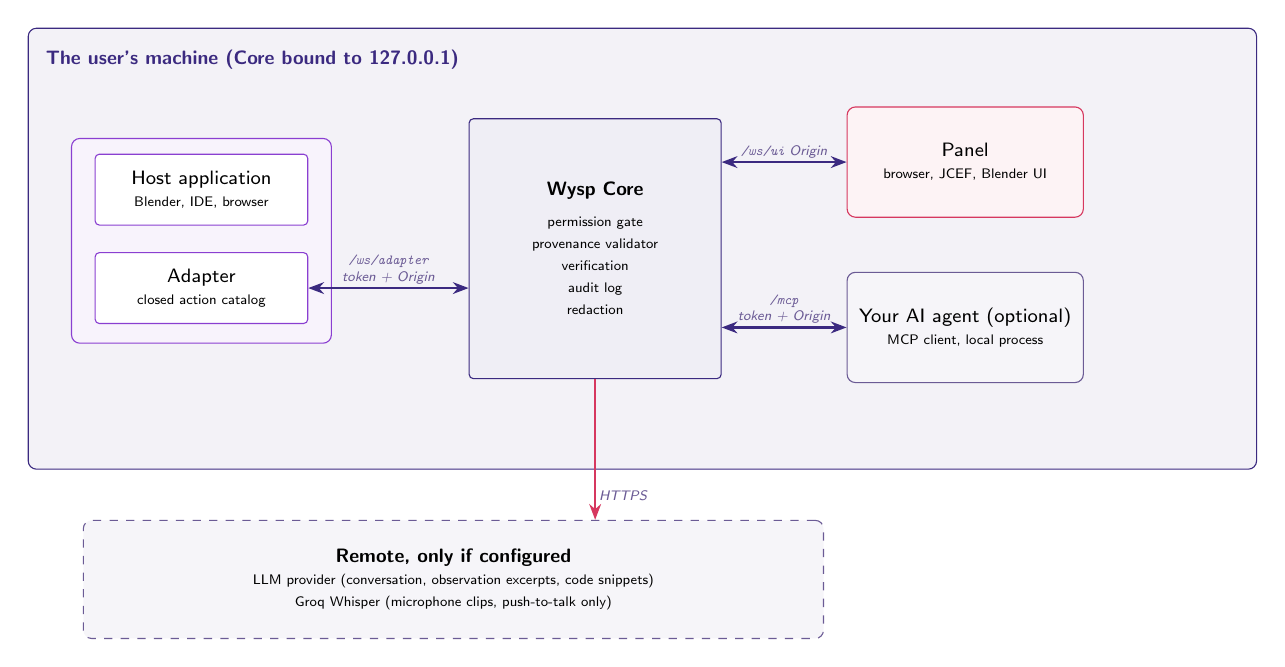
\begin{tikzpicture}[fig]
  \node[zone=inkpurple, minimum width=15.6cm, minimum height=5.6cm] (local) at (0,0.2) {};
  \node[font=\sffamily\bfseries\scriptsize, text=inkpurple, anchor=north west] at (-7.7,2.85) {The user's machine (Core bound to 127.0.0.1)};
  \node[zone=lilacdeep, minimum width=3.3cm, minimum height=2.6cm] (host) at (-5.6,0.3) {};
  \node[mod, minimum width=2.7cm, minimum height=0.9cm] (app) at (-5.6,0.95) {Host application\\\tiny Blender, IDE, browser};
  \node[mod, minimum width=2.7cm, minimum height=0.9cm] (adp) at (-5.6,-0.3) {Adapter\\\tiny closed action catalog};
  \node[mod, draw=inkpurple, fill=inkpurple!8, minimum width=3.2cm, minimum height=3.3cm, align=center] (core) at (-0.6,0.2) {\textbf{Wysp Core}\\[3pt]\tiny permission gate\\\tiny provenance validator\\\tiny verification\\\tiny audit log\\\tiny redaction};
  \node[zone=pinkdeep, minimum width=3.0cm, minimum height=1.4cm] (pn) at (4.1,1.3) {};
  \node[font=\sffamily\scriptsize] at (4.1,1.3) {Panel\\\tiny browser, JCEF, Blender UI};
  \node[zone=muted, minimum width=3.0cm, minimum height=1.4cm] (ag) at (4.1,-0.8) {};
  \node[font=\sffamily\scriptsize, align=center] at (4.1,-0.8) {Your AI agent (optional)\\\tiny MCP client, local process};
  \node[zone=muted, minimum width=9.4cm, minimum height=1.5cm, dashed] (cloud) at (-2.4,-4.0) {};
  \node[font=\sffamily\scriptsize, align=center] at (-2.4,-4.0) {\textbf{Remote, only if configured}\\\tiny LLM provider (conversation, observation excerpts, code snippets)\\\tiny Groq Whisper (microphone clips, push-to-talk only)};
  \draw[biarr] (adp.east) -- node[lab, above, align=center] {\code{/ws/adapter}\\token + Origin} (core.west |- adp.east);
  \draw[biarr] (core.east |- pn.west) -- node[lab, above] {\code{/ws/ui} Origin} (pn.west);
  \draw[biarr] (core.east |- ag.west) -- node[lab, above, align=center] {\code{/mcp}\\token + Origin} (ag.west);
  \draw[arr, color=pinkdeep] (core.south) -- ++(0,-1.1) -- node[lab, right, pos=0.55] {HTTPS} (cloud.north -| core.south);
\end{tikzpicture}
\caption{Zones and channels. The adapter, the Panel and the agent are separate clients of the Core. Only the dashed zone leaves the machine, and only when the user configured it.}\label{fig:boundaries}
\end{figure}

\begin{xltabular}{\textwidth}{@{}L{3.2cm}L{3.9cm}Y@{}}
\toprule
\textbf{Channel} & \textbf{Protection} & \textbf{Notes} \\
\midrule
\code{WS /ws/adapter} & Pairing token in \code{wysp.hello}; Origin allowlist & Token is \code{~/.wysp/token}, 32 random bytes, created once. A missing Origin (native clients) is allowed. \\
\code{WS /ws/ui} & Origin allowlist & No token. The first Panel is elected as the one that speaks. \\
\code{POST /api/listen/*} & Origin and token header \code{x-wysp-token} & Turns the microphone on, so it needs the token. \\
\code{POST /api/tts}, \code{/api/ocr} & Origin allowlist & Local voice and local text recognition only. No proxying of URLs. \\
\code{/mcp} & Token (Bearer or \code{X-Wysp-Token}), Origin, loopback host check & Served in external mode, or with \code{--mcp}. \\
\bottomrule
\end{xltabular}

The Origin allowlist contains the Core's own origin, the Panel dev server, and anything listed in \code{WYSP\_ALLOWED\_ORIGINS} (the Chrome extension's origin, for instance). The CLI refuses to bind to a non-loopback address unless \code{--unsafe-bind} is given.

\subsection{The data flow of a turn}\label{sec:turn}

A \emph{turn} starts when the user sends a message and ends when Wysp has finished answering. Figure~\ref{fig:turn} shows the six stages, and the list below explains what the code does in each.

\begin{figure}[H]
\centering
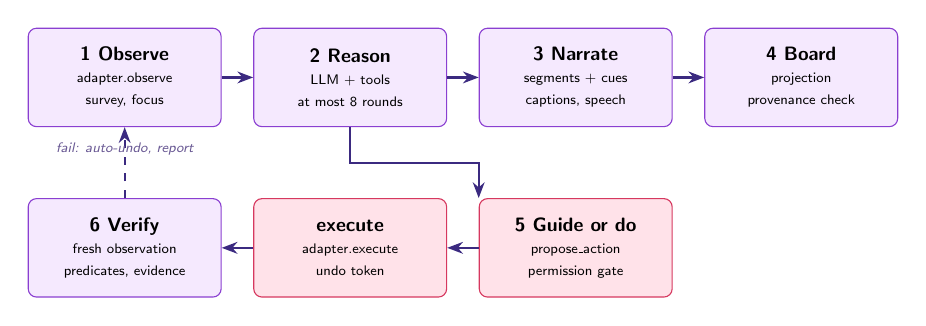
\begin{tikzpicture}[fig, node distance=4mm]
  \tikzset{st/.style={draw=lilacdeep, fill=lilac!18, rounded corners=3pt, minimum width=2.45cm, minimum height=1.25cm, align=center, inner sep=3pt}}
  \node[st] (o) {\textbf{1 Observe}\\\tiny adapter.observe\\\tiny survey, focus};
  \node[st, right=of o] (r) {\textbf{2 Reason}\\\tiny LLM + tools\\\tiny at most 8 rounds};
  \node[st, right=of r] (n) {\textbf{3 Narrate}\\\tiny segments + cues\\\tiny captions, speech};
  \node[st, right=of n] (b) {\textbf{4 Board}\\\tiny projection\\\tiny provenance check};
  \node[st, below=9mm of n, fill=pink!22, draw=pinkdeep] (g) {\textbf{5 Guide or do}\\\tiny propose\_action\\\tiny permission gate};
  \node[st, left=of g, fill=pink!22, draw=pinkdeep] (e) {\textbf{execute}\\\tiny adapter.execute\\\tiny undo token};
  \node[st, left=of e] (v) {\textbf{6 Verify}\\\tiny fresh observation\\\tiny predicates, evidence};
  \draw[arr] (o) -- (r); \draw[arr] (r) -- (n); \draw[arr] (n) -- (b);
  \draw[arr] (r.south) |- ($(r.south)+(0,-0.45)$) -| (g.north west);
  \draw[arr] (g) -- (e); \draw[arr] (e) -- (v);
  \draw[arr, dashed] (v.north) -- ++(0,0.5) -| node[lab, above, pos=0.2] {fail: auto-undo, report} (o.south);
\end{tikzpicture}
\caption{One turn. Lilac stages run in the Core's own logic; pink stages go through the permission gate and the adapter. The verify stage feeds its result back to the conversation.}\label{fig:turn}
\end{figure}

\begin{enumerate}[leftmargin=1.4em]
  \item \textbf{Observe.} When an adapter becomes the active one, the survey runs: the Core fetches the action catalog, the context and one full observation, and keeps a bounded summary (at most 4000 characters in the prompt). For each turn the system prompt also carries a fresh observation of the focus (up to 20 entities). Sensitive entities are counted, never named.
  \item \textbf{Reason.} The orchestrator builds the messages (system prompt, the last 12 history messages, the user text) and calls the language model with the tools that the adapter's capabilities allow. It loops for at most 8 rounds. A transient LLM error is retried once after 1.5 s. If the model writes a tool call as prose, the Core tries to recover it. Plain text from the model is narrated, so models that skip the \code{narrate} tool still work.
  \item \textbf{Narrate.} Speech is cut into segments of at most 300 characters. A segment can carry \emph{cues} (``at word 7, focus this node'') so that the board follows the voice. If the user interrupts, unplayed segments are kept and can be resumed.
  \item \textbf{Board.} \code{show\_entities} does not let the model write nodes. The Core \emph{projects} the observed entities the model selected, and the provenance validator downgrades any \pobs{} node without a matching ref in this session's observations. The Panel receives a patch.
  \item \textbf{Guide or do.} \code{propose\_action} validates the parameters against the action's JSON Schema. In guide mode the Core installs a watch with the action's postconditions, highlights the target in the application and waits for the user. In do mode the Core asks the permission gate, shows a dry-run preview and, if approved, executes.
  \item \textbf{Verify.} The Core observes again, evaluates the postconditions and produces \emph{evidence}. If the postconditions fail after a Wysp action, the Core undoes it and reports the failure.
\end{enumerate}

\begin{wherebox}
\file{core/src/wysp\_core/app.py} (endpoints, Origin allowlist), \file{gateway/server.py} (handshake, heartbeat), \file{orchestrator/turn.py} (turn loop), \file{orchestrator/context.py} (prompt), \file{orchestrator/pipeline.py} (guide, do, verify, undo). Specs: \file{.kiro/specs/core-orchestrator/}.
\end{wherebox}




\section{Inside the Core}\label{sec:core}

The Core is the package \file{core/src/wysp\_core/}. This chapter follows its modules in the order a request meets them. Figure~\ref{fig:coremap} gives the map.

\begin{figure}[H]
\centering
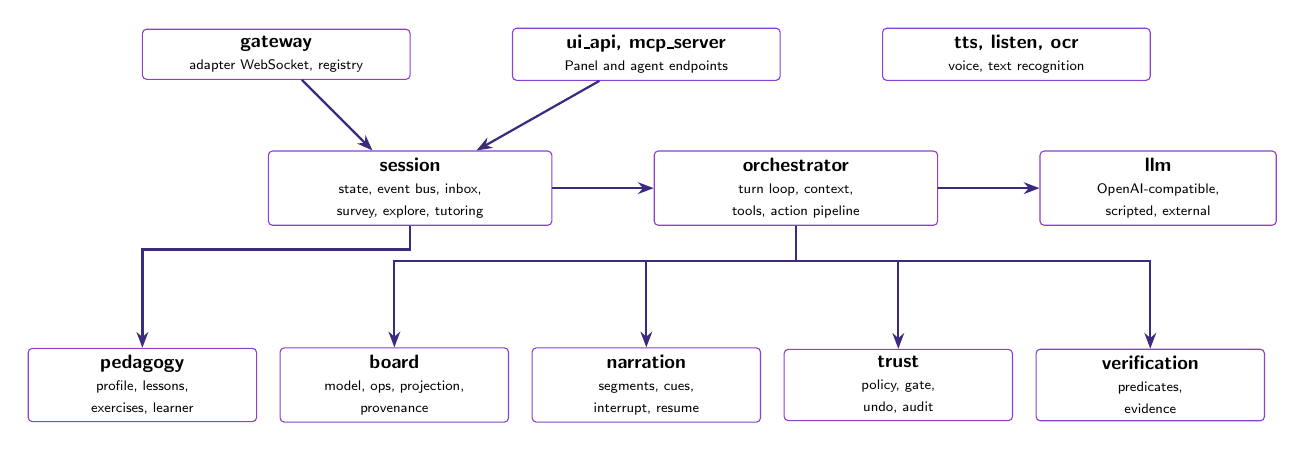
\begin{tikzpicture}[fig]
  \node[mod, minimum width=3.4cm] (gw) at (-4.7,2.9) {\textbf{gateway}\\\tiny adapter WebSocket, registry};
  \node[mod, minimum width=3.4cm] (ui) at (0,2.9) {\textbf{ui\_api, mcp\_server}\\\tiny Panel and agent endpoints};
  \node[mod, minimum width=3.4cm] (voice) at (4.7,2.9) {\textbf{tts, listen, ocr}\\\tiny voice, text recognition};
  \node[mod, minimum width=3.6cm] (sess) at (-3.0,1.2) {\textbf{session}\\\tiny state, event bus, inbox,\\\tiny survey, explore, tutoring};
  \node[mod, minimum width=3.6cm] (orch) at (1.9,1.2) {\textbf{orchestrator}\\\tiny turn loop, context,\\\tiny tools, action pipeline};
  \node[mod, minimum width=3.0cm] (llm) at (6.5,1.2) {\textbf{llm}\\\tiny OpenAI-compatible,\\\tiny scripted, external};
  \node[mod, minimum width=2.9cm] (ped) at (-6.4,-1.3) {\textbf{pedagogy}\\\tiny profile, lessons,\\\tiny exercises, learner};
  \node[mod, minimum width=2.9cm] (board) at (-3.2,-1.3) {\textbf{board}\\\tiny model, ops, projection,\\\tiny provenance};
  \node[mod, minimum width=2.9cm] (nar) at (0,-1.3) {\textbf{narration}\\\tiny segments, cues,\\\tiny interrupt, resume};
  \node[mod, minimum width=2.9cm] (trust) at (3.2,-1.3) {\textbf{trust}\\\tiny policy, gate,\\\tiny undo, audit};
  \node[mod, minimum width=2.9cm] (ver) at (6.4,-1.3) {\textbf{verification}\\\tiny predicates,\\\tiny evidence};
  \draw[arr] (gw) -- (sess); \draw[arr] (ui) -- (sess); \draw[arr] (sess) -- (orch); \draw[arr] (orch) -- (llm);
  \draw[thick, color=inkpurple] (orch.south) -- ++(0,-0.45);
  \foreach \c in {board, nar, trust, ver} \draw[arr] ($(orch.south)+(0,-0.45)$) -| (\c.north);
  \draw[arr] (sess.south) -- ++(0,-0.3) -| (ped.north);
\end{tikzpicture}
\caption{Core modules. Arrows show the main direction of calls; verification results feed the learner model in \code{pedagogy}. \code{contract/} (the models) is imported by all of them, and \code{store/} and \code{telemetry/} hold local files and logs.}\label{fig:coremap}
\end{figure}

\subsection{Session and gateway}

\textbf{Gateway.} \code{wysp.hello} must arrive within 10 s. The Core checks the token, validates the manifest, and compares only the \emph{major} contract version (a mismatch is error \code{-32018}). It answers with the heartbeat interval (20 s) and drops an adapter that is silent for 45 s. A new connection with the same adapter id replaces the old one. Requests to an adapter use the contract's time budgets plus a 1 s slack.

\textbf{Session.} One session object holds the active adapter, the board, the narration state, the permission gate, the undo stack, the conversation history and the learner model. Adapter events go onto an event bus. Events that arrive during a Wysp action, or within 1.5 s after it, are forced to \code{origin: wysp}, so that a Wysp change is never credited to the learner. Several adapters can be connected; the Panel chooses the active one (\code{adapter.activate}).

\subsection{Orchestrator and tools}

The language model sees 21 tools. Tools that need an adapter capability are offered only when the manifest declares it (property CORE-P10), and the call is refused again at run time.

\begin{xltabular}{\textwidth}{@{}L{3.2cm}Y@{}}
\toprule
\textbf{Group} & \textbf{Tools} \\
\midrule
Look & \code{observe} (levels summary, focus, full; optional root ref), \code{lookup\_concept} (glossary from the profile) \\
Show & \code{show\_entities}, \code{add\_concept} (\pinf{} or \pill{} nodes only), \code{annotate}, \code{narrate} (segments, cues, and a board update in one call), \code{highlight}, \code{clear\_highlight} \\
Act & \code{propose\_action} (mode \code{guide} or \code{do}; never runs anything by itself) \\
Teach & \code{learner\_status}, \code{lesson} (start, next, skip, repeat, stop), \code{start\_exercise}, \code{exercise\_hint}, \code{check\_exercise}, \code{declare\_done} \\
Explore & \code{code\_map}, \code{get\_study\_plan}, \code{study\_read}, \code{record\_understanding}, \code{finish\_study} \\
Ask & \code{ask\_clarification} (one short question with up to four options; ends the turn) \\
\bottomrule
\end{xltabular}

The system prompt is generic (\file{orchestrator/prompts/system.md}). App knowledge enters through the manifest (name, entity kinds, ref scheme), the profile's primer, the action catalog with risk levels, the current context fenced as \code{<app\_data>}, the survey, and the board labels with their provenance. Text found in an application is data, not instructions.

\subsection{Board and provenance}

The board model has nodes (id, ref, kind, label, provenance, confidence, a few properties to display), edges, ordered steps with a status (pending, active, done, failed) and annotations. A \emph{board op} changes it; there are twelve (add or remove node, edge or annotation, set layout, set focus, set or update steps, mark stale, clear). Ops apply atomically: a batch that would exceed 60 nodes or reference a missing node leaves the board untouched.

\textbf{Projection} turns an observation into nodes and edges deterministically (property CORE-P12). The node id is \code{n:<ref>}, the displayed properties come from the profile's \code{board.props} for that kind, and the board is re-projected when the application changes, dropping nodes that disappeared.

\textbf{Provenance validator.} Applied to every patch the model can influence. An \pobs{} node whose ref was not seen in an observation of this session is downgraded to \pinf{} and its ref is removed. An \pobs{} annotation is always downgraded. \code{add\_concept} forces non-observed provenance on its own, so the model has no path to create an observed fact.

\subsection{Narration}

Text is stripped of markdown and packed into segments of at most 300 characters. Each segment has a provenance, which the Panel shows as a marker (``likely'' for \pinf, ``for example'' for \pill). Only the Panel that was elected as the speaker drives the timeline, so two open Panels do not read every sentence twice. Text that looks like a tool call is never spoken.

\subsection{Permission gate, undo and audit}\label{sec:gate}

\begin{xltabular}{\textwidth}{@{}L{2.8cm}L{4.6cm}Y@{}}
\toprule
\textbf{Risk} & \textbf{Policy} & \textbf{Approval} \\
\midrule
\code{read\_only}, \code{ui\_state} & Run automatically, logged & none \\
\code{reversible} & Ask, unless a grant covers this action & Click, voice (``yes''), or ``allow for this lesson'' (a session grant for that action id) \\
\code{irreversible} & Ask with a preview; denied at integration level \code{visual} & Explicit click only. A voice answer is refused. \\
\bottomrule
\end{xltabular}

A pending request times out after 60 s and counts as denied. A new user message cancels pending requests. For reversible and irreversible actions the Core first runs the action with \code{dry\_run: true} so that the dialog can show a preview (for a text edit, a diff).

\textbf{Undo.} Every reversible action returns an undo token. The Core keeps a per-adapter stack of 50 records. The user can undo the last one (\code{undo.last}). If post-conditions fail after execution, the Core undoes the action by itself and tells the model the action was \code{failed\_and\_undone}.

\textbf{Audit.} Every proposal, decision (with who and how: click, voice, grant, policy or timeout), execution, verification, undo and guided step is appended to \file{\textasciitilde/.wysp/audit/YYYY-MM-DD.jsonl}. Records pass through a redactor that removes the pairing token, configured API keys and key-shaped strings, and long strings are truncated.

\subsection{Verification and the predicate language}

All verification uses one language, evaluated by the Core and never by the model. A \emph{comparison} is \code{\{ref?, path, op, value\}}, where \code{path} is a JMESPath expression run on the observation (or on one entity when \code{ref} is given) and \code{op} is one of \code{eq, ne, gt, gte, lt, lte, in, contains, exists, not\_exists, matches, len\_eq, len\_gte}. Comparisons combine with \code{all}, \code{any} and \code{not}.

\begin{lstlisting}[language={}]
{"all": [
  {"path": "entities[?kind=='modifier' && parent=='${params.target}' && props.type=='BEVEL'] | length(@)",
   "op": "gte", "value": 1}]}
\end{lstlisting}

Placeholders (\code{\$\{params.x\}}, \code{\$\{bindings.x\}}) are substituted only in allowed positions. Inside a JMESPath string literal the value is escaped, and values containing a backslash or a control character are rejected, which prevents a parameter from injecting expression syntax (CON-P11). \code{matches} uses a full match with a pattern limit of 200 characters. To verify, the Core always takes a \emph{fresh} full observation, evaluates the predicates and builds an \code{Evidence} record from the outcomes (actual and expected value per comparison, observation id, state version, timestamp).

\subsection{Pedagogy}

\textbf{Profile.} \file{profile.yaml} (id, application name, languages, a primer for the model, skills with prerequisites and optional BKT parameters, speech hints and an optional \code{explore} section), \file{concepts.yaml} (the glossary) and \file{lessons/*.yaml}. \code{wysp validate-profile} checks required keys, duplicate ids, prerequisite cycles and lesson validity.

\textbf{Lessons and exercises.} A lesson has steps (\code{explain}, \code{show}, \code{guide}, \code{do}, \code{check}) and exercises. An exercise has a prompt, bindings (variables resolved from the context, for example the selected object), success predicates, ordered hints and a maximum number of attempts. The Core \emph{offers} an exercise only if its bindings resolve and its success predicate is not already true. The model may phrase the prompt but never invents success criteria. The Core evaluates the exercise when the application changes.

\textbf{Evidence and mastery.} Evidence is \code{verified} (predicate true on a fresh observation after a user action, weight 1.0), \code{answered} (weight 0.6, reserved in the contract) or \code{declared} (the learner says it is done and the application cannot verify it, weight 0.3, refused for verifiable exercises). Each hint lowers the weight by 15\%, down to 40\% of it. The learner model is a simplified Bayesian Knowledge Tracing per skill (defaults: slip 0.1, guess 0.2, transit 0.15, prior 0.2), written atomically to \file{\textasciitilde/.wysp/learners/<profile>.json}. A correct answer never lowers mastery. The tutor adapts depth: below 0.4 basics, below 0.85 guided practice, from 0.85 a challenge. \emph{An event whose origin is} \code{wysp} \emph{never counts}: four separate checks enforce it (PED-P4).

\subsection{Survey and exploration}

The \emph{survey} runs when an adapter becomes active. It stays in memory, goes stale on any state change, refreshes after 2 s, and retries with backoff when the application is busy (for example an IDE that is indexing). If a full observation takes too long it falls back to a summary.

\emph{Exploration} is for large structured applications such as a codebase. It exists only if the profile has an \code{explore} section, and nothing is read until the user presses Start in the Panel (consent). The Core then builds a \emph{code map} without any model, by walking subtree observations: names, signatures, sizes and dependencies, not code bodies. Limits: 4000 adapter calls, 300 s, 60\,000 entries. It also ranks about 30 files to read first. The study phase (\code{study\_read}, \code{record\_understanding}, \code{finish\_study}) records what was actually read; \code{finish\_study} is refused below 80\% read coverage, and files not read are marked unread so the tutor does not claim to know them. The study is started automatically only in external-agent mode; with the Core's own model, the map is available through \code{code\_map} and the tutor reads files on request. Notes are saved per project under \file{\textasciitilde/.wysp/projects/}.

\subsection{LLM providers and external mode}\label{sec:core-llm}

The Core talks to any OpenAI-compatible endpoint with tool calling, without streaming. Presets: Groq, Cerebras, OpenRouter, Pollinations (keyless fallback), OpenAI and Ollama, or any URL through \code{WYSP\_LLM\_BASE\_URL}. With \code{--llm auto}, the first of Groq, Cerebras and OpenRouter whose key is set is used, otherwise Pollinations. The provider retries on 429 (honouring \code{Retry-After}, capped at 20 s), 5xx and timeouts. \code{--llm scripted} replays a YAML scenario and is what the automated tests and the offline demo use.

\textbf{External mode} (\code{wysp serve --llm external}) removes the model from the Core. The Core serves an authenticated MCP endpoint at \code{/mcp} with the same 21 tools plus \code{get\_tutor\_context} (the rules and the application description) and \code{wait\_for\_user} (messages and interruptions from the Panel, up to 55 s). The user's own agent, such as Kiro, Claude Code or any MCP client, does the thinking. Board, voice, permission gate and verification stay in Wysp, and every tool call goes through the same \code{ToolBox}, so an agent can never create an observed node or approve its own action. For clients that only speak stdio, \code{wysp mcp-bridge} forwards to the running Core; by default it is read-only (\code{observe}, \code{lookup\_concept}, \code{get\_tutor\_context}, \code{wait\_for\_user}, \code{code\_map}, \code{get\_study\_plan}, \code{study\_read}, \code{learner\_status}) and refuses any URL that is not loopback.

\subsection{Voice}

Speech output is offline: Windows voices through SAPI, or Kokoro (an 82M-parameter neural voice, Apache-2.0, installed with \code{wysp install-voice}). Output text is capped at 600 characters per request. Speech input is push-to-talk: hold Space in the Panel (Web Speech API when the browser has it), or Alt+Space in Blender. When the browser cannot listen, the Core records the microphone between \code{/api/listen/start} and \code{/stop} (at most 30 s, kept in memory, silence is never sent) and transcribes with Whisper on Groq. That clip leaves the machine; \code{WYSP\_STT\_PROVIDER=none} turns it off. Windows text recognition (\code{/api/ocr}) is local and is used to find a label in a screenshot of an application's own interface.

\subsection{Logs}

Each Core session writes a JSONL log to \file{\textasciitilde/.wysp/logs/} at level \code{off}, \code{basic} (timings, counts, errors) or \code{full} (default, adds conversation text and tool arguments). \code{wysp logs list|summary|timeline} reads them. The level can change from the Panel.

\begin{wherebox}
\file{core/src/wysp\_core/}: \file{session/}, \file{orchestrator/}, \file{board/}, \file{narration/}, \file{trust/}, \file{verification/}, \file{pedagogy/}, \file{llm/}, \file{mcp\_server/}, \file{tts.py}, \file{listen.py}. Specs: \file{.kiro/specs/core-orchestrator/}, \file{.kiro/specs/pedagogy-verification/}. Agent mode: \file{docs/agent-mode.md}.
\end{wherebox}



\section{The adapter contract and the three tutors}\label{sec:adapters}

\subsection{Transport and session}

The adapter is the WebSocket \emph{client} and the Core is the \emph{server} at \code{ws://127.0.0.1:8765/ws/adapter}. This suits hosts that can open outgoing connections but would struggle to listen (Blender's embedded Python, a Chrome service worker). Messages are JSON-RPC 2.0 in both directions on one connection.

\begin{enumerate}[leftmargin=1.4em]
  \item The adapter sends \code{wysp.hello \{manifest, token\}}. The Core checks the token, the manifest and the major contract version.
  \item The adapter sends \code{wysp.heartbeat} at least every 20 s. The Core does not ping; it disconnects an adapter that has been silent for 45 s.
  \item The Core sends \code{adapter.*} requests. The adapter sends \code{event.*} notifications.
\end{enumerate}

{\small
\begin{xltabular}{\textwidth}{@{}L{4.9cm}L{3.4cm}L{3.0cm}Y@{}}
\toprule
\textbf{Method} & \textbf{Result} & \textbf{Capability} & \textbf{Budget} \\
\midrule
\code{adapter.observe} & Observation & \code{observe} & 1 s \\
\code{adapter.get\_context} & Context ($\leq$ 8 KB) & \code{context} & 0.5 s \\
\code{adapter.get\_actions} & ActionSpec list & \code{actions} & 0.5 s \\
\code{adapter.execute} & ActionResult, undo token & \code{execute} & 5 s \\
\code{adapter.undo} & ActionResult & \code{undo} & 5 s \\
\code{adapter.highlight} & ok & \code{highlight} & 0.5 s \\
\code{adapter.clear\_highlight} (1.1) & \code{\{cleared\}} & \code{highlight} & 0.5 s \\
\code{adapter.verify} & Evidence list & \code{verify.native} & 2 s \\
\midrule
\code{event.state\_changed} & \multicolumn{3}{>{\raggedright\arraybackslash}X}{\code{\{state\_version, changed[], origin\}}; capability \code{events.state}} \\
\code{event.selection\_changed} & \multicolumn{3}{>{\raggedright\arraybackslash}X}{\code{\{focus[]\}}; capability \code{events.selection}} \\
\code{event.user\_action} & \multicolumn{3}{>{\raggedright\arraybackslash}X}{\code{\{kind, target, details, origin\}}; capability \code{events.user\_action}} \\
\code{event.navigation} & \multicolumn{3}{>{\raggedright\arraybackslash}X}{\code{\{url, title\}}; capability \code{events.navigation}} \\
\code{event.highlight\_dismissed} (1.1) & \multicolumn{3}{>{\raggedright\arraybackslash}X}{\code{\{ref, reason\}}: the user touched the highlighted thing} \\
\bottomrule
\end{xltabular}}

Parameters: \code{observe \{scope\}} with a level (summary, focus, full), an optional root ref and a depth; \code{execute \{call\}} with action id, params, request id and \code{dry\_run}; \code{undo \{token\}}; \code{highlight \{ref, style, duration\_ms\}}.

Capabilities are promises: the Core calls only what the manifest declares. \code{observe}, \code{context} and \code{actions} are required. The core of the contract is deliberately small. Most adapters implement \code{observe}, \code{get\_context}, \code{get\_actions}, \code{execute}, \code{undo} and \code{highlight}, and verification is done by the Core on fresh observations, so no adapter re-implements verification logic. \code{adapter.verify} exists for cases where a native check is more reliable.

\subsection{The observation model}

An observation is an \emph{entity graph}: \code{entities[]} (\code{ref}, \code{kind}, \code{label}, \code{parent}, \code{props}, \code{confidence}), \code{links[]}, \code{focus[]}, \code{truncated} and \code{counts}. The Core knows no kinds in advance. Each adapter declares its kinds in the manifest, and the contract kit checks that every kind used is declared.

\begin{lstlisting}[language={}]
{"observation_id": "o-118", "state_version": 42, "scope": {"level": "focus"},
 "entities": [
  {"ref": "blender://object/Pumpkin", "kind": "object", "label": "Pumpkin",
   "props": {"type": "MESH", "modifiers_count": 2}},
  {"ref": "blender://object/Pumpkin/modifier/Solidify", "kind": "modifier",
   "label": "Solidify", "parent": "blender://object/Pumpkin",
   "props": {"type": "SOLIDIFY", "index": 1, "thickness": 0.02}}],
 "links": [], "focus": ["blender://object/Pumpkin"], "truncated": false}
\end{lstlisting}

Limits: 500 entities and 256 KB per observation, 8 KB for the context, refs matching \code{scheme://...} up to 512 characters. When an adapter cuts an observation it sets \code{truncated} and reports true totals in \code{counts}, and the tutor is told so it does not claim a list is complete. Entities whose \code{props.sensitive} is true are counted but never named.

The \textbf{state digest} (SHA-256 of canonical JSON over entities and links, without volatile properties, floats rounded to 6 significant digits) defines ``the state is unchanged'': an invalid call must leave it equal, and undo must restore it. Each adapter lists its own volatile properties in the manifest.

\subsection{Actions, risk levels and postconditions}

An adapter publishes a \emph{closed, declarative} catalog. An action declares an id (\code{verb\_object}), a description written for the model, a JSON Schema for its parameters (\code{additionalProperties: false}), a risk level, a \code{reversible} flag consistent with the risk, optional preconditions, \emph{postconditions} (predicates with \code{\$\{params.*\}} placeholders), and optionally \code{guide.ui\_path}, the steps the user would follow in the interface. Risk levels and their policy are in \cref{sec:gate}. An action that evaluates arbitrary code (Python \code{exec}, JavaScript injection, a shell command, an arbitrary IDE action id) is forbidden, and the kit rejects ids that look like it.

Execution rules every adapter follows: validate parameters before touching anything; support \code{dry\_run} (return a preview, change nothing, return no undo token); return an \code{undo\_token} for reversible actions and make \code{adapter.undo} restore the same digest; tag changes caused by Wysp with \code{origin: wysp} so the Core never credits them to the learner. Errors use the standard JSON-RPC codes plus \code{-32010} to \code{-32019} (not supported, action not found, target not found, precondition failed, execution failed, undo unavailable, timeout, busy, incompatible version, unauthorized).

\subsection{Persistent highlights (contract 1.1)}

\code{adapter.highlight} points at an entity or at an interface element the adapter documents (for example \code{intellij://ui/label/Commit}). Version 1.1 added \code{duration\_ms: 0}, meaning ``until cleared'', the request \code{adapter.clear\_highlight} and the notification \code{event.highlight\_dismissed}. An adapter keeps at most one highlight, removes it when the user interacts with the target (ignoring caret moves and scrolls its own highlight caused) and when the connection drops. The Core ends a persistent highlight when the tutor clears it, replaces it, a guided step is verified, the adapter disconnects, or after 10 minutes. With an adapter that declares 1.0, the Core falls back to a timed highlight.

\subsection{Versioning and generated artefacts}

\code{contract\_version} is 1.1.0. Additive, optional changes bump the minor version; breaking changes bump the major version. The Core accepts any adapter with the same major version. The Pydantic models are the source of truth: \code{uv run python -m wysp\_core.contract.export} writes the JSON Schemas to \file{schemas/} (26 schemas and an index) and the TypeScript types to \file{sdk/ts/src/generated/}. CI fails if the committed files differ from a fresh export. Neither directory is edited by hand.

\subsection{How to write an adapter}

The guide \file{docs/\allowbreak adapter-guide.md} builds a complete adapter for a toy notes application (\file{sdk/python/\allowbreak examples/\allowbreak notes\_adapter.py}, tested against the Core's own models). In short:

\begin{enumerate}[leftmargin=1.4em]
  \item \textbf{Manifest}: id, integration level, ref scheme, capabilities, entity kinds, volatile properties, profile id.
  \item \textbf{Observation}: map the application state to entities with stable refs. The Python SDK (\code{AdapterRuntime}) gives you the client, the state version and the routing; you implement \code{observe} and \code{get\_context}. In TypeScript, \code{@wysp/adapter-sdk} provides the client and \code{defineAction}.
  \item \textbf{Actions}: one file per action with schema, risk, postconditions and UI path.
  \item \textbf{Profile}: skills, concepts, lessons and exercises in YAML.
  \item \textbf{Check}: \code{uv run wysp-contract --tutor <name>} (\cref{sec:kit}).
\end{enumerate}

\subsection{What is application-specific}

\begin{figure}[H]
\centering
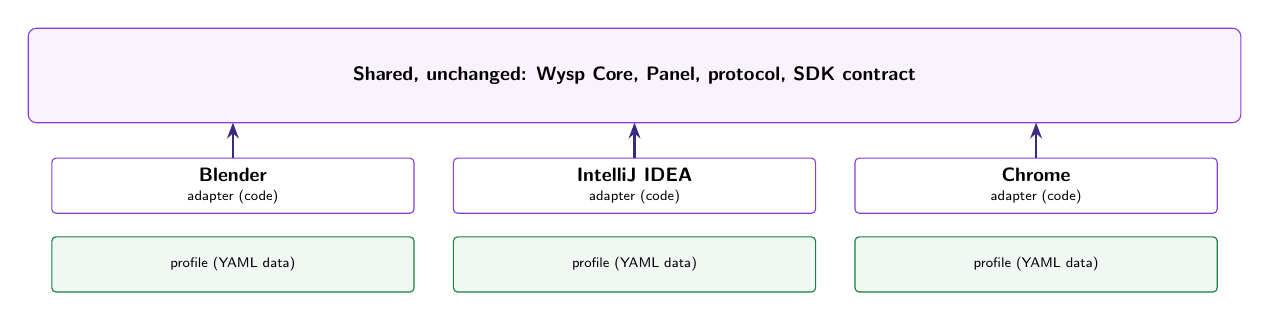
\begin{tikzpicture}[fig]
  \node[zone=lilacdeep, minimum width=15.4cm, minimum height=1.2cm, align=center] (core) at (0,2.2) {\textbf{Shared, unchanged: Wysp Core, Panel, protocol, SDK contract}};
  \foreach \x/\t in {-5.1/Blender, 0/IntelliJ IDEA, 5.1/Chrome} {
    \node[mod, minimum width=4.6cm, minimum height=0.7cm] at (\x,0.8) {\textbf{\t}\\[-1pt]\tiny adapter (code)};
    \node[mod, draw=okgreen, fill=okgreen!6, minimum width=4.6cm, minimum height=0.7cm] at (\x,-0.2) {\tiny profile (YAML data)};
  }
  \draw[arr] (-5.1,1.15) -- (-5.1,1.6); \draw[arr] (0,1.15) -- (0,1.6); \draw[arr] (5.1,1.15) -- (5.1,1.6);
\end{tikzpicture}
\caption{Adding a tutor changes only the two lower rows.}\label{fig:appspecific}
\end{figure}

\begin{xltabular}{\textwidth}{@{}L{2.4cm}Y Y Y@{}}
\toprule
 & \textbf{Blender} & \textbf{IntelliJ IDEA} & \textbf{Chrome (optional)} \\
\midrule
Code & Python extension, \code{bpy}; Blender 5.2 LTS & Kotlin plugin on the IntelliJ Platform 2026.2; no third-party runtime dependency & TypeScript, Manifest V3, Chrome 116 or later \\
Integration & \code{native} & \code{native} & \code{interface} \\
Ref scheme & \code{blender://} & \code{intellij://} & \code{web://} \\
Entity kinds & scene, collection, object, modifier, material & project, module, directory, file, symbol, problem, run configuration & page, region, heading, form, control, dialog, table, list, chart, status \\
Threading rule & Never touch \code{bpy} off the main thread. The network thread queues requests, a \code{bpy.app.timers} pump (every 50 ms) runs them. & Read the model in non-blocking read actions on pooled threads. Change code only in write commands on the EDT. Swing only on the EDT. & The WebSocket lives in the service worker (heartbeat 20 s keeps it alive). DOM work happens in the content script. \\
Undo & Blender's own undo history gets a step after each change, so Ctrl+Z also works. & Each change is one IDE command (``Wysp: ...''), read back after writing, restored if wrong. Wysp's undo never overwrites newer typing. & Undo tokens are stored in \code{storage.session}. \\
Pointing & GPU overlays: pulsing box on objects, frame and callout on editors, regions and Properties tabs. & Editor markup, a glass-pane painter and balloons; label positions come from Swing. & A closed shadow-DOM overlay in lilac that respects reduced motion. \\
\bottomrule
\end{xltabular}

\subsection{Blender}

The adapter runs inside Blender as an extension (\file{blender\_manifest.toml}, id \code{wysp\_tutor}, Blender 5.2 or later, GPL-3.0-or-later as Blender add-ons require) with two bundled pure-Python wheels: the adapter SDK and \code{websocket-client}. A depsgraph handler only marks the scene dirty; the main-thread loop diffs per-entity hashes (at most every 250 ms) and emits one \code{event.state\_changed}. Around each action the adapter flushes the diff before and after, so what the action changed is tagged \code{wysp} and everything else \code{user}. Blender cannot capture audio, so its panel uses the Core's \code{/api/listen/*} and \code{/api/tts} and plays the audio with \code{aud}.

Inside Blender the interface is native: a sidebar panel with the chat, an approval card and a viewport banner, and a node-tree view of the board (\code{.Wysp Board}, removed before the file is saved). It speaks the same \code{/ws/ui} protocol as the browser Panel, which is how a different UI technology still counts as the same Panel protocol. Actions (10): \code{select\_object}, \code{show\_properties\_tab} (\code{ui\_state}); \code{set\_object\_transform}, \code{add\_modifier}, \code{set\_modifier\_property}, \code{move\_modifier}, \code{toggle\_modifier\_visibility}, \code{assign\_material}, \code{remove\_modifier} (\code{reversible}); \code{apply\_modifier} (\code{irreversible}). Profile: 3 lessons, 4 skills, 12 concepts.

\subsection{IntelliJ IDEA}

The plugin connects with \code{java.net.http.WebSocket} and a small JSON codec, and embeds the Core's Panel in a tool window through JCEF (when JCEF is missing, the tool window links to the browser). The pairing token travels in the URL fragment, so no server ever sees it. Symbols come from the IDE's structure view, and imports (Java, Kotlin, Python) give the dependency edges used by exploration. While the IDE indexes, symbols are marked pending and the adapter sends \code{event.state\_changed} when indexing ends.

Actions (13): \code{open\_file}, \code{go\_to\_symbol}, \code{show\_tool\_window} (\code{ui\_state}); \code{read\_code}, \code{search\_code}, \code{find\_usages}, \code{list\_files} (\code{read\_only}, with caps such as 150 lines or 50 matches per call); \code{rename\_symbol}, \code{replace\_lines}, \code{insert\_lines}, \code{create\_file}, \code{reformat\_code}, \code{optimize\_imports} (\code{reversible}). Nothing runs code, run configurations or arbitrary IDE action ids. Sensitive files (\code{.env*}, keys, certificates, files named like credentials or secrets) are never read or written, by file name. Code text reaches the Core only for the selection (1500 characters), the code at the caret (3000) and read-tool results (8000 per call). Profile: 2 lessons, 6 skills, 22 concepts and an \code{explore} section.

\subsection{Chrome}

The extension is optional and sits outside the main demo path. It is active only on allowlisted origins (default \code{http://localhost:5180}, matched exactly), requested as optional host permissions per origin. The user pastes the pairing token into the options page. The content script builds an accessibility-oriented snapshot (roles and accessible names through \code{dom-accessibility-api}) and refs of the form \code{web://host/region\textasciitilde{}name/role\textasciitilde{}name}, rebuilt from the live DOM at execution time; an ambiguous target fails with up to five candidates.

\textbf{Redaction.} Values of password, hidden, card, one-time-code and \code{data-wysp-sensitive} fields are replaced with \code{[redacted]}; texts are cut at 200 characters; page URLs are sent without query or fragment; cookies, storage and request headers are never sent. Actions (7): \code{scroll\_into\_view}, \code{focus\_element}, \code{follow\_link} (\code{ui\_state}, same allowlisted site only); \code{fill\_field}, \code{select\_option}, \code{set\_checked} (\code{reversible}); \code{click\_element} (\code{irreversible}, with a dry-run preview). Profile: 3 lessons, 3 skills, 13 concepts.

\begin{wherebox}
\file{docs/adapter-guide.md}, \file{.kiro/specs/adapter-contract/}, \file{core/src/wysp\_core/contract/}, \file{schemas/}, \file{sdk/python/}, \file{sdk/ts/}. Tutors: \file{apps/blender-tutor/} (\file{adapter/runtime.py}, \file{adapter/actions/}), \file{apps/intellij-tutor/plugin/src/main/kotlin/dev/wysp/intellij/}, \file{apps/web-tutor/extension/src/}. Each has a \file{README.md} with its action table and privacy notes.
\end{wherebox}




\section{Key workflows}\label{sec:workflows}

Five sequences show how the pieces cooperate. Dashed arrows are replies. ``Core'' stands for the orchestrator, session, board and trust modules of \cref{sec:core}.

\subsection{Explain what is on screen}

The user asks a question. The Core takes a fresh observation, the model answers with one \code{narrate} call that carries the segments, cues and the refs to show, and the Core projects them onto the board.

\begin{figure}[H]
\centering
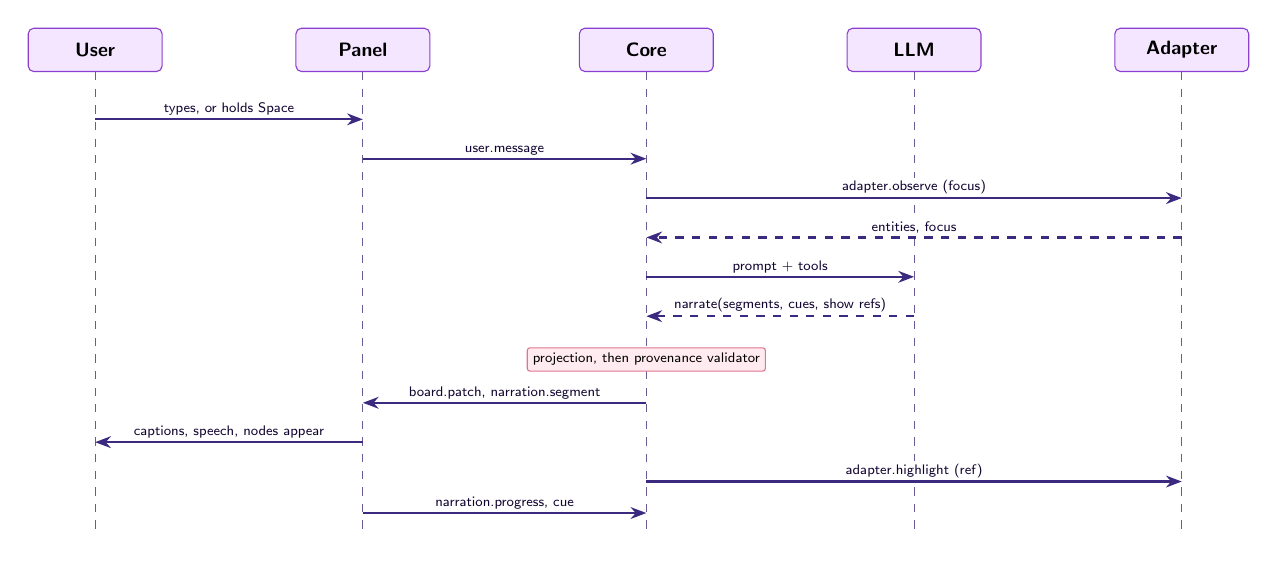
\begin{tikzpicture}[fig]
  \renewcommand{\seqlife}{5.9}
  \actor{U}{0}{User}\actor{P}{3.4}{Panel}\actor{C}{7.0}{Core}\actor{L}{10.4}{LLM}\actor{A}{13.8}{Adapter}
  \msg{U}{P}{0.6}{types, or holds Space}
  \msg{P}{C}{1.1}{user.message}
  \msg{C}{A}{1.6}{adapter.observe (focus)}
  \ret{A}{C}{2.1}{entities, focus}
  \msg{C}{L}{2.6}{prompt + tools}
  \ret{L}{C}{3.1}{narrate(segments, cues, show refs)}
  \note{C}{3.65}{projection, then provenance validator}
  \msg{C}{P}{4.2}{board.patch, narration.segment}
  \msg{P}{U}{4.7}{captions, speech, nodes appear}
  \msg{C}{A}{5.2}{adapter.highlight (ref)}
  \msg{P}{C}{5.6}{narration.progress, cue}
\end{tikzpicture}
\caption{Explain. The model never touches the board directly, and each cue moves the board focus while the speech plays.}\label{fig:wf-explain}
\end{figure}

\subsection{A guided step, verified}

In guide mode the user does the work. Wysp watches the application and verifies the postconditions when the user changes it.

\begin{figure}[H]
\centering
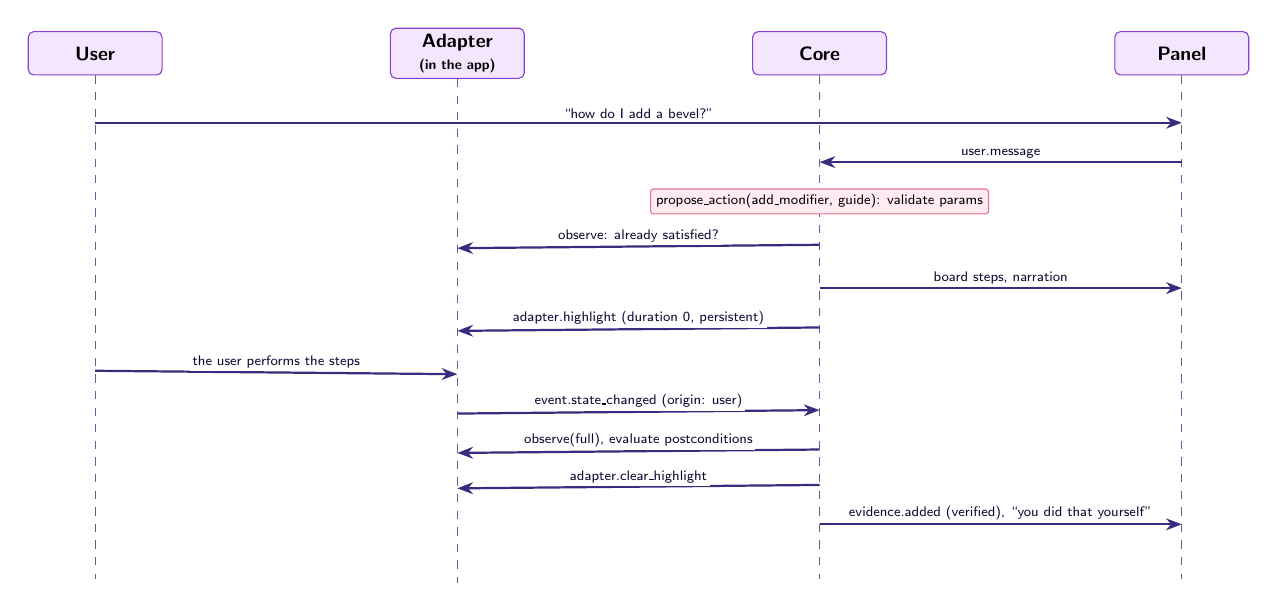
\begin{tikzpicture}[fig]
  \renewcommand{\seqlife}{6.4}
  \actor{U}{0}{User}\actor{A}{4.6}{Adapter\\\tiny (in the app)}\actor{C}{9.2}{Core}\actor{P}{13.8}{Panel}
  \msg{U}{P}{0.6}{``how do I add a bevel?''}
  \msg{P}{C}{1.1}{user.message}
  \note{C}{1.6}{propose\_action(add\_modifier, guide): validate params}
  \msg{C}{A}{2.15}{observe: already satisfied?}
  \msg{C}{P}{2.7}{board steps, narration}
  \msg{C}{A}{3.2}{adapter.highlight (duration 0, persistent)}
  \msg{U}{A}{3.75}{the user performs the steps}
  \msg{A}{C}{4.25}{event.state\_changed (origin: user)}
  \msg{C}{A}{4.75}{observe(full), evaluate postconditions}
  \msg{C}{A}{5.2}{adapter.clear\_highlight}
  \msg{C}{P}{5.7}{evidence.added (verified), ``you did that yourself''}
\end{tikzpicture}
\caption{Guide. The step turns green only after the predicates hold on a fresh observation. Events with origin \code{wysp} never close a guided step as the user's achievement.}\label{fig:wf-guide}
\end{figure}

\subsection{An approved action, with undo}

\begin{figure}[H]
\centering
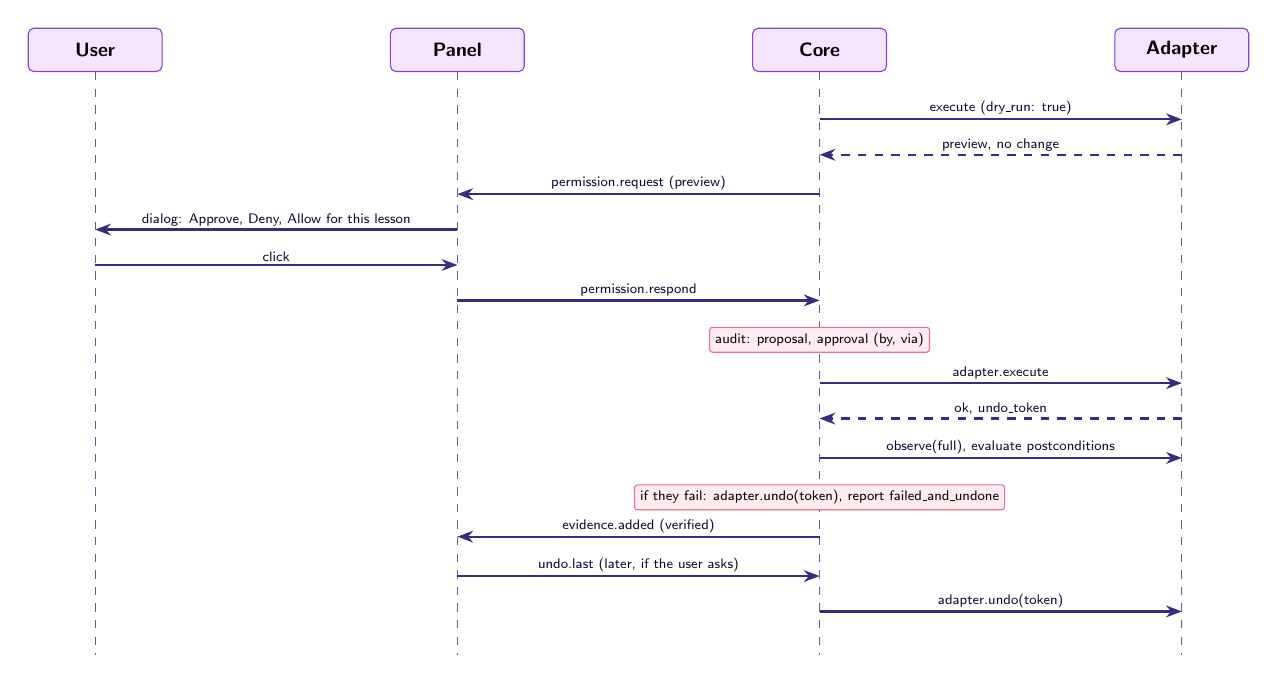
\begin{tikzpicture}[fig]
  \renewcommand{\seqlife}{7.4}
  \actor{U}{0}{User}\actor{P}{4.6}{Panel}\actor{C}{9.2}{Core}\actor{A}{13.8}{Adapter}
  \msg{C}{A}{0.6}{execute (dry\_run: true)}
  \ret{A}{C}{1.05}{preview, no change}
  \msg{C}{P}{1.55}{permission.request (preview)}
  \msg{P}{U}{2.0}{dialog: Approve, Deny, Allow for this lesson}
  \msg{U}{P}{2.45}{click}
  \msg{P}{C}{2.9}{permission.respond}
  \note{C}{3.4}{audit: proposal, approval (by, via)}
  \msg{C}{A}{3.95}{adapter.execute}
  \ret{A}{C}{4.4}{ok, undo\_token}
  \msg{C}{A}{4.9}{observe(full), evaluate postconditions}
  \note{C}{5.4}{if they fail: adapter.undo(token), report failed\_and\_undone}
  \msg{C}{P}{5.9}{evidence.added (verified)}
  \msg{P}{C}{6.4}{undo.last (later, if the user asks)}
  \msg{C}{A}{6.85}{adapter.undo(token)}
\end{tikzpicture}
\caption{Do. A voice ``yes'' may approve a reversible action; an irreversible action needs a click and the Core refuses any other channel.}\label{fig:wf-do}
\end{figure}

\subsection{An exercise with evidence}

\begin{figure}[H]
\centering
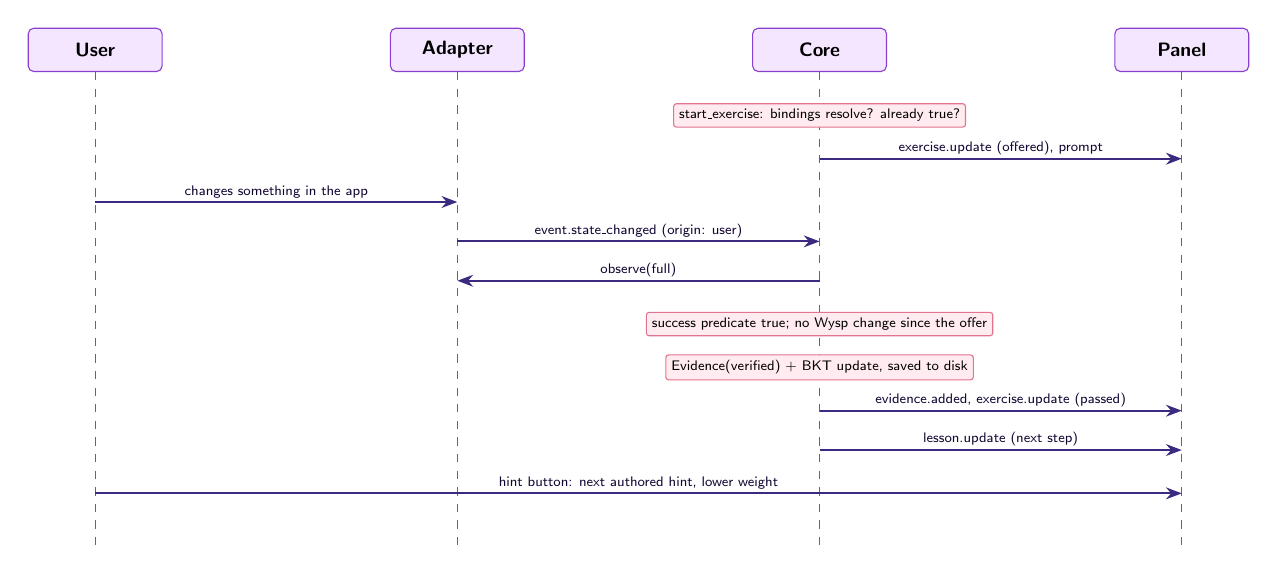
\begin{tikzpicture}[fig]
  \renewcommand{\seqlife}{6.0}
  \actor{U}{0}{User}\actor{A}{4.6}{Adapter}\actor{C}{9.2}{Core}\actor{P}{13.8}{Panel}
  \note{C}{0.55}{start\_exercise: bindings resolve? already true?}
  \msg{C}{P}{1.1}{exercise.update (offered), prompt}
  \msg{U}{A}{1.65}{changes something in the app}
  \msg{A}{C}{2.15}{event.state\_changed (origin: user)}
  \msg{C}{A}{2.65}{observe(full)}
  \note{C}{3.2}{success predicate true; no Wysp change since the offer}
  \note{C}{3.75}{Evidence(verified) + BKT update, saved to disk}
  \msg{C}{P}{4.3}{evidence.added, exercise.update (passed)}
  \msg{C}{P}{4.8}{lesson.update (next step)}
  \msg{U}{P}{5.35}{hint button: next authored hint, lower weight}
\end{tikzpicture}
\caption{Exercise. The success criteria are authored predicates. The model phrases the prompt but never judges the result.}\label{fig:wf-exercise}
\end{figure}

If the learner says ``I'm done'' before the predicate holds, the Core verifies right then and counts it as an attempt. If the application cannot verify the exercise, \code{declare\_done} records \code{declared} evidence at weight 0.3, and the Panel labels it as declared rather than verified.

\subsection{Exploration and study of a project}

\begin{figure}[H]
\centering
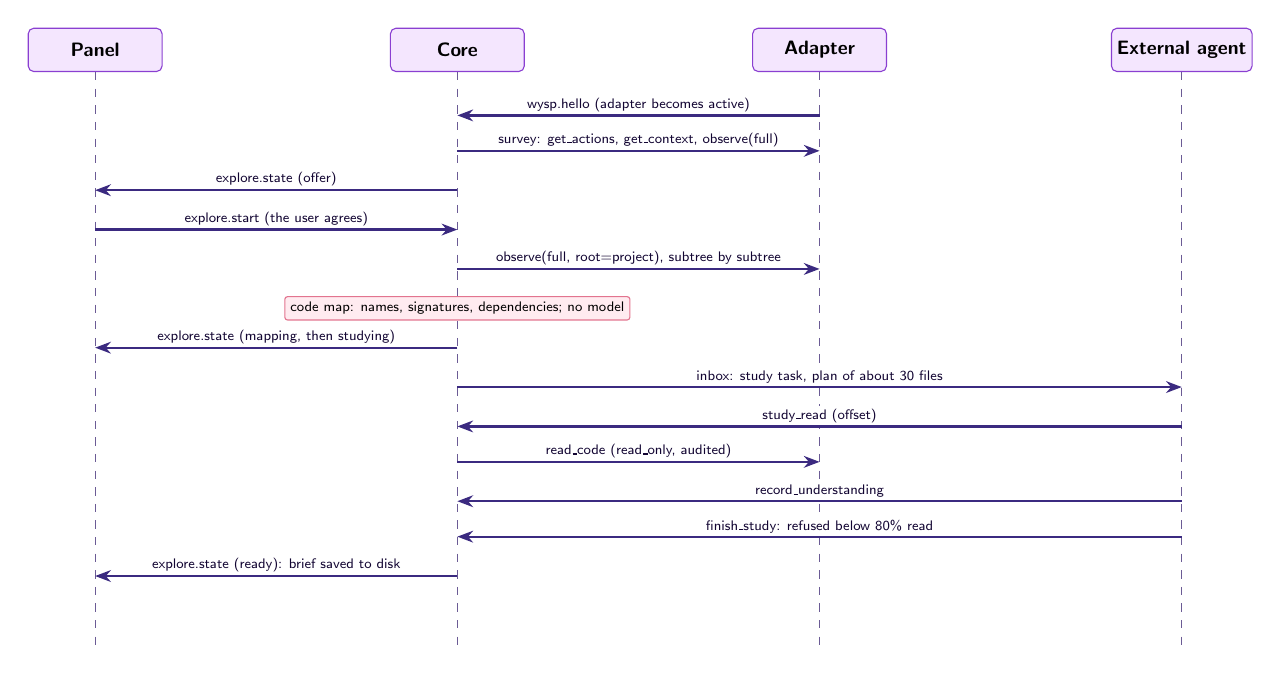
\begin{tikzpicture}[fig]
  \renewcommand{\seqlife}{7.3}
  \actor{P}{0}{Panel}\actor{C}{4.6}{Core}\actor{A}{9.2}{Adapter}\actor{G}{13.8}{External agent}
  \msg{A}{C}{0.55}{wysp.hello (adapter becomes active)}
  \msg{C}{A}{1.0}{survey: get\_actions, get\_context, observe(full)}
  \msg{C}{P}{1.5}{explore.state (offer)}
  \msg{P}{C}{2.0}{explore.start (the user agrees)}
  \msg{C}{A}{2.5}{observe(full, root=project), subtree by subtree}
  \note{C}{3.0}{code map: names, signatures, dependencies; no model}
  \msg{C}{P}{3.5}{explore.state (mapping, then studying)}
  \msg{C}{G}{4.0}{inbox: study task, plan of about 30 files}
  \msg{G}{C}{4.5}{study\_read (offset)}
  \msg{C}{A}{4.95}{read\_code (read\_only, audited)}
  \msg{G}{C}{5.45}{record\_understanding}
  \msg{G}{C}{5.9}{finish\_study: refused below 80\% read}
  \msg{C}{P}{6.4}{explore.state (ready): brief saved to disk}
\end{tikzpicture}
\caption{Exploration. Nothing is read before the user agrees. The study loop is shown with an external agent; with the Core's own model the map is available through \code{code\_map} and the tutor reads files on request.}\label{fig:wf-explore}
\end{figure}

\begin{wherebox}
\file{core/src/wysp\_core/orchestrator/pipeline.py} (guide, do, verify, undo), \file{pedagogy/exercises.py}, \file{session/survey.py}, \file{session/explore.py}. End-to-end tests of these flows run against the mock adapter: \file{contract-tests/tests/test\_core\_with\_mock.py}, \file{test\_explore.py}, \file{test\_survey.py}.
\end{wherebox}


\section{How Kiro was used}\label{sec:kiro}

Kiro is used in two directions: to \emph{build} Wysp, and as one of the possible \emph{brains} of a running tutor. Everything below is in the repository under \file{.kiro/}.

\subsection{Building Wysp with Kiro}

\begin{xltabular}{\textwidth}{@{}L{2.5cm}Y@{}}
\toprule
\textbf{Feature} & \textbf{What we did with it} \\
\midrule
Specs & Seven specs, each with EARS requirements, a design with numbered correctness properties, and tasks: \code{adapter-contract}, \code{core-orchestrator}, \code{pedagogy-verification}, \code{tutor-panel}, \code{blender-tutor}, \code{intellij-tutor} and \code{web-tutor} (the optional extra). Together 80 requirements and 132 tasks. Changes went spec first: contract 1.1.0 was written in the contract spec before any code used persistent highlights, and the exploration feature started as a requirement in \code{core-orchestrator}. \\
Steering & Ten files. Always loaded: product vocabulary, structure and boundary rules, technology stack, testing rules, trust and safety. Loaded when matching files are open: the adapter contract guide, the Panel design system, pedagogy. On demand: demo and release checklists. \\
Hooks & Ten hooks in three files, all calling \file{scripts/kiro/hook.py}, which CI runs too: a core boundary guard, schema sync, offline contract check, a trust review of changes to actions and manifests, a new-action integration prompt, formatting, profile validation and tests after each task. \\
Agents & Three specialist agents: \code{blender-adapter}, \code{browser-adapter} and a read-only \code{contract-guardian} that reviews a change against the contract, the boundary rules and the trust rules. A fourth, \code{wysp-tutor}, is the tutor loop (below). \\
MCP & Context7 for current library documentation and Playwright for browser checks. \code{wysp mcp-bridge} gives Kiro a read-only stdio view of a running tutor. \\
\bottomrule
\end{xltabular}

\textbf{Property tests come from spec properties.} Each design lists correctness properties (58 in total, such as ``CON-P6: undo restores the state digest'' or ``CORE-P2: the model cannot create observed facts''). Each one is implemented as a property-based test, with Hypothesis in Python and fast-check in TypeScript, and cites its id in the test name. This is a testing rule in the steering, not an option.

\textbf{Live sessions feed the journal.} \file{docs/kiro-journal.md} records what Kiro produced, what we changed, and what a spec, hook or test caught. Examples recorded there: the boundary hook flagged application words in a new log analyser; the IDE's slow-operation check caught work on the wrong thread, which led to a three-phase execution in the IntelliJ adapter; a live run showed the Core crediting the learner for a step Wysp had done itself, was reproduced on the mock adapter first and fixed in the Core; and a log of a study session showed the tutor describing an architecture after three file reads, which led to the code map, read-coverage tracking and the 80\% rule.

\subsection{Kiro as the tutor's brain}

\begin{figure}[H]
\centering
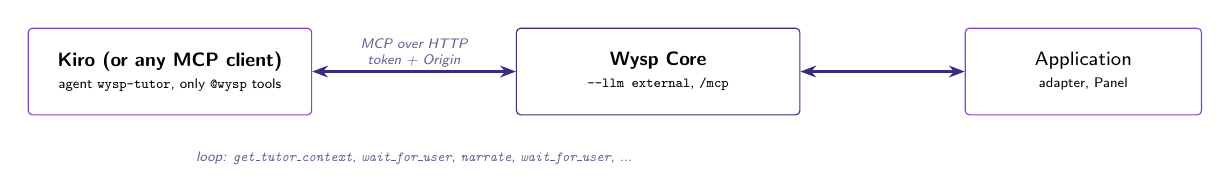
\begin{tikzpicture}[fig]
  \node[mod, minimum width=3.6cm, minimum height=1.1cm] (k) at (0,0) {\textbf{Kiro (or any MCP client)}\\\tiny agent \code{wysp-tutor}, only \code{@wysp} tools};
  \node[mod, minimum width=3.6cm, minimum height=1.1cm, draw=inkpurple] (c) at (6.2,0) {\textbf{Wysp Core}\\\tiny \code{--llm external}, \code{/mcp}};
  \node[mod, minimum width=3.0cm, minimum height=1.1cm] (a) at (11.6,0) {Application\\\tiny adapter, Panel};
  \draw[biarr] (k) -- node[lab, above, align=center] {MCP over HTTP\\token + Origin} (c);
  \draw[biarr] (c) -- (a);
  \node[lab, align=center] at (3.1,-1.1) {loop: \code{get\_tutor\_context}, \code{wait\_for\_user}, \code{narrate}, \code{wait\_for\_user}, ...};
\end{tikzpicture}
\caption{External mode: Kiro does the thinking, Wysp is the body (board, voice, permission gate, verification).}\label{fig:kiro-brain}
\end{figure}

The agent file \file{.kiro/agents/wysp-tutor.json} connects to the Core's MCP endpoint, has no file or shell tools, and can change the project only through \code{propose\_action}, which goes through the permission gate. \file{scripts/kiro\_tutor.ps1} restarts it each turn with \code{kiro-cli chat --agent wysp-tutor}, because an agent that ends its model turn would otherwise go idle. The same endpoint works for Claude Code or any MCP client (\file{docs/agent-mode.md}).

\begin{wherebox}
\file{.kiro/specs/}, \file{.kiro/steering/}, \file{.kiro/hooks/}, \file{.kiro/agents/}, \file{.kiro/settings/mcp.json}, \file{docs/kiro/mcp.example.json}, \file{docs/kiro-journal.md}, \file{scripts/kiro/hook.py}, \file{.github/workflows/ci.yml}.
\end{wherebox}


\section{Trust, safety, privacy and testing}\label{sec:trust}

\subsection{The trust model}

\begin{enumerate}[leftmargin=1.4em]
  \item \textbf{Provenance.} Every board element and factual claim is \pobs, \pinf{} or \pill. An \pobs{} node must reference an entity ref present in an observation recorded in the current session; otherwise the validator downgrades it to \pinf{} and logs it. Observed nodes are created by projection in Core code, never written by the model. At the \code{visual} integration level observations carry a confidence below 1, and the Panel shows it.
  \item \textbf{Actions need permission.} The model has one way to act, \code{propose\_action}. Execution goes permission gate, then adapter, then post-condition verification (\cref{sec:gate}). A failed verification triggers an automatic undo.
  \item \textbf{Closed action catalogs.} Each adapter declares its actions. No action runs arbitrary code, and the contract kit rejects action ids that look like \code{exec}, \code{eval}, \code{shell} or \code{script}.
  \item \textbf{Achievements count only the user.} Events with \code{origin: wysp} never count as evidence of mastery.
  \item \textbf{Page and scene content is data.} Text found in an application, a web page or a file never changes the tutor's rules. The permission gate is the last barrier against prompt injection, because even a fully fooled model can only propose.
  \item \textbf{Audit.} Every proposal, decision, execution, verification and undo is appended to \file{\textasciitilde/.wysp/\allowbreak audit/*.jsonl}.
\end{enumerate}

\subsection{Local security and privacy}

The Core binds to \code{127.0.0.1} (the CLI refuses another host without \code{--unsafe-bind}). Adapters authenticate with the pairing token, browser-origin WebSocket upgrades are checked against the Origin allowlist, there is no CORS wildcard, and no endpoint proxies arbitrary URLs. Tokens and API keys are redacted from audit records, error snippets and warnings, and are never logged. The Chrome extension is active only on allowlisted origins, and the IntelliJ plugin never reads sensitive files (\cref{sec:adapters}).

\begin{xltabular}{\textwidth}{@{}L{4.3cm}L{4.4cm}Y@{}}
\toprule
\textbf{What} & \textbf{Where it goes} & \textbf{Control} \\
\midrule
Conversation text, observation excerpts, code snippets (IntelliJ), entity names & The configured LLM provider, which may be remote (Groq, Cerebras, OpenRouter, Pollinations, OpenAI) or local (Ollama) & Choose a provider; \code{--llm scripted} or \code{ollama} keep everything local; sensitive entities are counted but not named \\
Microphone clip (push-to-talk, at most 30 s, never silence) & Groq Whisper, in memory only, nothing stored & \code{WYSP\_STT\_PROVIDER=none} \\
Speech output & Local Windows voices or Kokoro, no network after the one-time model download & \code{WYSP\_TTS\_PROVIDER=none} \\
Screenshot of an application's own interface (label finding) & Local Core, processed in memory by Windows text recognition, not stored & Local only \\
Session logs & \file{\textasciitilde/.wysp/logs/} on disk & \code{WYSP\_LOG=off\textbar basic\textbar full} \\
Page snapshots (Chrome) & Local Core; passwords, card, one-time-code and hidden fields are replaced by \code{[redacted]}, text cut at 200 characters, no cookies, storage or headers & Allowlisted origins only \\
\bottomrule
\end{xltabular}

\subsection{Testing strategy}\label{sec:testing}

Every component is testable without the real application, using the mock adapter, a scripted LLM provider and recorded fixtures. Automated tests never call a real LLM, STT or TTS provider. A bug fix starts with a failing test. Anything that needs Blender, Chrome or the IDE is marked \code{live} and runs on demand.

\begin{xltabular}{\textwidth}{@{}L{3.1cm}L{4.1cm}Y@{}}
\toprule
\textbf{Layer} & \textbf{Tooling} & \textbf{Scope} \\
\midrule
Unit & pytest, Vitest, JUnit & Per package. \\
Property-based & Hypothesis, fast-check & Test names start with \code{test\_prop\_} or \code{prop:} and cite the property id. \\
Contract kit & \code{wysp-contract} & The same checks run against the mock adapter and the real tutors. \\
Golden fixtures & JSON in \file{contract-tests/\allowbreak fixtures/} & Valid and invalid protocol messages and board patches that Python and TypeScript must treat identically. \\
Live & pytest \code{-m live}, Playwright, IDE harness & Real Blender, Chromium with the extension, a sandbox IDE. \\
\bottomrule
\end{xltabular}

On the day of writing, \code{uv run pytest --collect-only} collects 371 Python tests by default (core 124, contract kit and mock 133, SDK 15, Blender tutor 99) and deselects 14 live tests. The TypeScript suites contain about 130 test cases in 21 files (Panel, SDK, Chrome extension), and the IntelliJ plugin has five Kotlin test files with about 50 tests, of which the platform tests need the IDE.

\subsubsection{Correctness properties}

Each spec lists numbered properties. All 58 ids appear in at least one test.

\begin{xltabular}{\textwidth}{@{}L{1.2cm}Y@{}}
\toprule
\textbf{Family} & \textbf{Properties} \\
\midrule
CON (11) & P1 schema round trip; P2 observation referential integrity; P3 ref and digest stability; P4 digest invariance; P5 invalid calls leave state unchanged; P6 undo round trip; P7 postconditions hold; P8 monotonic state version; P9 origin tagging; P10 size limits; P11 safe placeholder substitution \\
CORE (16) & P1 provenance soundness; P2 the model cannot create observed facts; P3 patch convergence; P4 gate policy; P5 audit completeness; P6 verify or undo; P7 interruption; P8 resume; P9 board size bound; P10 tools follow capabilities; P11 redaction; P12 projection determinism; P13 survey provenance; P14 survey bounded and non-blocking; P15 code map bounded and honest; P16 a study entry never claims an unread file \\
PED (9) & P1 mastery bounded; P2 correct verified evidence never lowers mastery; P3 evidence strength ordered; P4 Wysp actions never count; P5 no stale success; P6 offers need resolved bindings; P7 profile validity; P8 hints in order; P9 recommendation respects prerequisites \\
PAN (6) & P1 patch parity with the Core; P2 gap detection; P3 layout determinism; P4 narration order and cancellation; P5 no voice approval for irreversible actions; P6 provenance style total and distinct \\
BLD (6) & P1 main-thread confinement; P2 compensating undo; P3 modifier projection total; P4 origin tagging; P5 debounce; P6 board mirror \\
IJ (4+1) & P1 codec round trip; P2 refs round trip; P3 sensitive files never leak; P4 rename is undoable (a fifth, ``edits and undos round trip'', exists in the tests) \\
WEB (6) & P1 redaction; P2 locator round trip; P3 ref stability; P4 overlay invisibility; P5 origin tagging; P6 allowlist enforcement \\
\bottomrule
\end{xltabular}

\subsubsection{The Contract Test Kit}\label{sec:kit}

\code{wysp-contract} plays the Core's part towards an adapter. It starts a throw-away WebSocket server on a free port with its own token (your Core and \file{\textasciitilde/.wysp} are not touched), starts the tutor as its \file{contract.fixture.yaml} says, and runs fifteen checks in order: \code{connect}, \code{manifest}, \code{context}, \code{observe\_integrity}, \code{ref\_stability}, \code{min\_entities}, \code{action\_catalog}, \code{postconditions}, \code{undo\_round\_trip}, \code{dry\_run}, \code{invalid\_calls}, \code{state\_version}, \code{events}, \code{highlight} and \code{latency}. It can write JUnit XML and a JSON recording of every message with tokens removed. \code{--offline} validates the fixture and the latest recording against the current models in seconds, which is what CI runs for the tutors.

\textbf{Fault injection.} The mock adapter can be started with a deliberate bug, and the kit must then fail with exit code 1: \code{wrong\_origin}, \code{undo\_noop}, \code{undeclared\_kind}, \code{postcondition\_lie}, \code{state\_version\_regression}, \code{dirty\_invalid}, \code{dry\_run\_mutates} and \code{unstable\_digest}. This tests the tester: a kit that passes a broken adapter would be worse than none.

\textbf{CI} (GitHub Actions, four jobs): the Python job (ruff, the Core boundary check, generated schemas up to date, profile validation, the kit offline for both main tutors, pytest); the contract-kit job (online on the mock adapter, a run with 300 ms of injected latency, and the fault-injection runs); the Panel job (typecheck, tests, build); and the TypeScript SDK job (generated types up to date, typecheck, tests). The Chrome extension tests run locally. The online runs against Blender, Chrome and IntelliJ are not in CI because they need the applications.

\begin{wherebox}
\file{.kiro/steering/trust-and-safety.md}, \file{.kiro/steering/testing.md}, \file{core/src/wysp\_core/trust/}, \file{board/provenance.py}, \file{store/redact.py}, \file{contract-tests/} (\file{wysp\_contract/online.py}, \file{wysp\_mock/faults.py}), \file{.github/workflows/ci.yml}, each tutor's README for its privacy notes.
\end{wherebox}



\section{Limits and roadmap}\label{sec:limits}

Wysp is a working prototype built in a few weeks. This chapter lists what it does not do, or does only partly, so that nobody has to discover it by accident.

\subsection{Known limits}

\begin{itemize}[leftmargin=1.2em]
  \item \textbf{Windows first.} Offline speech output uses Windows SAPI or Kokoro, and label finding in screenshots uses Windows text recognition. The Core, the contract and the Panel are not Windows-specific, but the voice and recognition paths have been exercised only on Windows. The dev scripts are PowerShell.
  \item \textbf{Local trust, not a sandbox.} The Core trusts processes on the same machine to the degree the pairing token and the Origin allowlist allow. \code{/ws/ui}, \code{/api/tts} and \code{/api/ocr} need no token (a client without an Origin header is accepted, as native clients must be), so any local process can drive the Panel protocol. The \code{via} field of a permission answer (click or voice) is reported by the Panel and is not independently verified by the Core. Adapters run inside the application with that application's privileges.
  \item \textbf{Model quality and latency.} The Core does not stream model output. Free hosted tiers are rate limited, and the keyless fallback (Pollinations) is slow and sometimes stalls. Quality depends on the model's tool calling. The scripted provider exists so that demos and tests do not depend on this.
  \item \textbf{One active application at a time.} Several adapters can be connected, but the tutor works with the active one.
  \item \textbf{Small boards.} The board holds at most 60 nodes, and observations at most 500 entities and 256 KB. Larger applications rely on \code{truncated}, \code{counts} and subtree observations.
  \item \textbf{Exploration depends on who thinks.} The study phase starts by itself only in external-agent mode. With the Core's own model, the code map is available and the tutor reads files on request.
  \item \textbf{Thin lesson content.} The profiles hold 3 lessons (Blender), 2 (IntelliJ) and 3 (Chrome). They prove the mechanism; they are not a curriculum.
  \item \textbf{Evidence types.} \code{answered} evidence (quiz answers) is defined in the contract and weighted by the learner model, but no part of the Core produces it yet.
  \item \textbf{The \code{visual} integration level is specified, not shipped.} The contract defines confidence below 1 and forbids irreversible actions there, but no tutor uses it as its integration level. The Blender tutor uses screenshots only to find the position of a label, locally.
  \item \textbf{Not everything runs in CI.} CI covers the Core, the contract kit on the mock adapter (with fault injection), the Panel and the TypeScript SDK. Blender, Chrome and IntelliJ runs need the applications and are run by hand (\code{pytest -m live}, the IDE harness).
  \item \textbf{Two licences.} The repository is MIT. The Blender extension is GPL-3.0-or-later, as Blender add-ons require.
  \item \textbf{Two Panel implementations of one protocol.} Browser, IntelliJ and Chrome show the React Panel. Blender shows a native interface that speaks the same \code{/ws/ui} protocol, so Blender-side UI changes are made twice.
\end{itemize}

\subsection{Roadmap}

These are directions that follow from the limits, not commitments.

\begin{itemize}[leftmargin=1.2em]
  \item More tutors through the SDK and the kit. A tutor for a document or spreadsheet application would test the \code{interface} level further. A visual-level adapter would exercise the confidence model.
  \item Produce \code{answered} evidence from short in-Panel questions.
  \item A token for \code{/ws/ui}, and verification of the approval channel, to tighten the local trust model.
  \item Streaming model output, so captions and speech start earlier.
  \item Cross-platform voice and text recognition.
  \item Run the online contract kit against Blender and Chrome in CI on a runner that has them.
  \item More lessons per profile, and a documented authoring workflow for profiles.
\end{itemize}

\begin{wherebox}
\file{README.md} (status), \file{docs/agent-mode.md} (limits of external mode), \file{.kiro/specs/*/tasks.md} (what is done and what is open), \file{docs/kiro-journal.md}.
\end{wherebox}


\section{Appendices}\label{sec:appendices}

\subsection{Repository map}

\begin{xltabular}{\textwidth}{@{}L{4.6cm}Y@{}}
\toprule
\textbf{Path} & \textbf{Content} \\
\midrule
\file{core/src/wysp\_core/} & The Core. \file{contract/} (models, export), \file{gateway/}, \file{ui\_api/}, \file{mcp\_server/}, \file{session/}, \file{orchestrator/}, \file{llm/}, \file{board/}, \file{narration/}, \file{pedagogy/}, \file{verification/}, \file{trust/}, \file{store/}, \file{telemetry/}, \file{cli.py} \\
\file{schemas/} & Generated JSON Schemas (never edited by hand) \\
\file{contract-tests/} & Contract Test Kit (\file{wysp\_contract/}), mock Kanban adapter (\file{wysp\_mock/}), fixtures \\
\file{sdk/python/}, \file{sdk/ts/} & Adapter SDKs; the TypeScript types in \file{sdk/ts/src/generated/} are generated \\
\file{panel/} & The React Panel \\
\file{apps/blender-tutor/} & \file{adapter/}, \file{profile/}, \file{demo/}, \file{contract.fixture.yaml} \\
\file{apps/intellij-tutor/} & \file{plugin/} (Kotlin, Gradle), \file{profile/}, \file{demo/sample-project/} \\
\file{apps/web-tutor/} & \file{extension/}, \file{profile/}, \file{demo-dashboard/} (optional third tutor) \\
\file{.kiro/} & Specs, steering, hooks, agents, MCP settings \\
\file{docs/} & \file{adapter-guide.md}, \file{agent-mode.md}, \file{kiro-journal.md}, \file{brand/}, this document in \file{architecture/} (French original in \file{architecture/fr/}) \\
\file{scripts/} & Dev scripts, brand asset generation, the Kiro hook dispatcher \file{kiro/hook.py} \\
\bottomrule
\end{xltabular}

\subsection{Commands}

Python 3.13 with uv and Node 24 are required. On Windows, use \code{npm.cmd} if PowerShell blocks \code{npm}.

\begin{xltabular}{\textwidth}{@{}L{5.0cm}Y@{}}
\toprule
\textbf{Goal} & \textbf{Command} \\
\midrule
Install & \code{uv sync}; \code{npm install}; \code{npm run build -w panel} \\
Two-minute demo (no application, no key) & \code{uv run wysp serve --llm scripted --scenario contract-tests/wysp\_mock/scenario.yaml}, then in a second terminal \code{uv run wysp-mock-adapter}, then open \url{http://127.0.0.1:8765} \\
Core with a hosted model & \code{uv run wysp serve} (keys in \file{.env}, see \file{.env.example}) \\
Core for your own agent & \code{uv run wysp serve --llm external}; \code{uv run wysp mcp-config} \\
Core and headless Blender & \code{scripts\textbackslash dev\_up.ps1 [-Llm scripted -Scenario file.yaml]}; \code{scripts\textbackslash dev\_down.ps1} \\
Build and install the Blender extension & \code{uv run python scripts\textbackslash build\_blender\_extension.py --install} \\
Build the IntelliJ plugin & \code{apps\textbackslash intellij-tutor\textbackslash plugin\textbackslash gradlew.bat buildPlugin} \\
Python tests & \code{uv run pytest}; live: \code{uv run pytest -m live -o addopts="" apps\textbackslash blender-tutor\textbackslash tests} \\
TypeScript tests & \code{npm test -w panel}; \code{npm test --workspaces --if-present} \\
Contract kit & \code{uv run wysp-contract --tutor blender-tutor [--offline]}; \code{--mock}; \code{--fixture contract-tests/fixtures/mock/contract.fixture.yaml [--fault NAME]} \\
Boundary check & \code{uv run --no-project python scripts/kiro/hook.py boundaries} \\
Regenerate schemas and types & \code{uv run python -m wysp\_core.contract.export} \\
Validate a profile & \code{uv run wysp validate-profile apps/blender-tutor/profile} \\
Logs & \code{uv run wysp logs list\textbar summary\textbar timeline} \\
Voice & \code{uv sync --all-packages --extra voice}; \code{uv run wysp install-voice}; \code{WYSP\_TTS\_PROVIDER=kokoro} \\
\bottomrule
\end{xltabular}

\subsection{Reference tables}

\subsubsection{Configuration (environment variables)}

\begin{xltabular}{\textwidth}{@{}L{5.0cm}Y@{}}
\toprule
\textbf{Variable} & \textbf{Effect} \\
\midrule
\code{WYSP\_LLM\_PROVIDER}, \code{WYSP\_LLM\_MODEL}, \code{WYSP\_LLM\_BASE\_URL}, \code{WYSP\_LLM\_API\_KEY} & Model provider (\code{groq}, \code{cerebras}, \code{openrouter}, \code{pollinations}, \code{openai}, \code{ollama}, or a custom URL). Preset keys: \code{GROQ\_API\_KEY}, \code{CEREBRAS\_API\_KEY}, \code{OPENROUTER\_API\_KEY}, \code{OPENAI\_API\_KEY}. \\
\code{WYSP\_TTS\_PROVIDER}, \code{WYSP\_TTS\_VOICE} & \code{auto}, \code{sapi}, \code{kokoro}, \code{none}; voice name \\
\code{WYSP\_STT\_PROVIDER}, \code{WYSP\_STT\_API\_KEY}, \code{WYSP\_STT\_MODEL} & \code{auto}, \code{groq}, \code{none}; Whisper model (default \code{whisper-large-v3-turbo}) \\
\code{WYSP\_OCR\_PROVIDER} & \code{auto} or \code{none} \\
\code{WYSP\_ALLOWED\_ORIGINS} & Extra allowed Origins, comma separated \\
\code{WYSP\_LOG} & \code{off}, \code{basic}, \code{full} (default) \\
\code{WYSP\_SURVEY} & \code{off} disables the survey \\
\code{WYSP\_HOME} & Replaces \file{\textasciitilde/.wysp} \\
\bottomrule
\end{xltabular}

\subsubsection{Action catalogs}

\begin{xltabular}{\textwidth}{@{}L{2.4cm}L{2.6cm}Y@{}}
\toprule
\textbf{Tutor} & \textbf{Risk} & \textbf{Actions} \\
\midrule
Mock Kanban & \code{read\_only} & \code{describe\_card} \\
 & \code{ui\_state} & \code{select\_card} \\
 & \code{reversible} & \code{create\_card}, \code{move\_card}, \code{rename\_card} \\
 & \code{irreversible} & \code{archive\_card} \\
\midrule
Blender & \code{ui\_state} & \code{select\_object}, \code{show\_properties\_tab} \\
 & \code{reversible} & \code{set\_object\_transform}, \code{add\_modifier}, \code{set\_modifier\_property}, \code{move\_modifier}, \code{toggle\_modifier\_visibility}, \code{assign\_material}, \code{remove\_modifier} \\
 & \code{irreversible} & \code{apply\_modifier} \\
\midrule
IntelliJ IDEA & \code{read\_only} & \code{read\_code}, \code{search\_code}, \code{find\_usages}, \code{list\_files} \\
 & \code{ui\_state} & \code{open\_file}, \code{go\_to\_symbol}, \code{show\_tool\_window} \\
 & \code{reversible} & \code{rename\_symbol}, \code{replace\_lines}, \code{insert\_lines}, \code{create\_file}, \code{reformat\_code}, \code{optimize\_imports} \\
\midrule
Chrome & \code{ui\_state} & \code{scroll\_into\_view}, \code{focus\_element}, \code{follow\_link} \\
 & \code{reversible} & \code{fill\_field}, \code{select\_option}, \code{set\_checked} \\
 & \code{irreversible} & \code{click\_element} \\
\bottomrule
\end{xltabular}

\subsubsection{Entity kinds and refs}

\begin{xltabular}{\textwidth}{@{}L{2.4cm}L{5.0cm}Y@{}}
\toprule
\textbf{Tutor} & \textbf{Kinds} & \textbf{Ref examples} \\
\midrule
Mock Kanban & board, column, card & \code{mock://...} \\
Blender & scene, collection, object, modifier, material & \code{blender://object/Candle}, \code{blender://object/Pumpkin/modifier/Solidify}, UI: \code{blender://ui/area/PROPERTIES} \\
IntelliJ & project, module, directory, file, symbol, problem, run\_config & \code{intellij://file/src/Main.java}, \code{intellij://file/path\#Class.member}, UI: \code{intellij://ui/toolwindow/Project}, \code{intellij://lines/path:12-20} \\
Chrome & page, region, heading, form, control, dialog, table, list, chart, status & \code{web://localhost:5180/\allowbreak region\textasciitilde{}filters/\allowbreak combobox\textasciitilde{}region} \\
\bottomrule
\end{xltabular}

\subsubsection{Panel protocol (\code{/ws/ui})}

\raggedright\textbf{Panel to Core} (14): \code{user.message}, \code{user.interrupt}, \code{user.continue}, \code{permission.respond}, \code{board.select}, \code{board.ask\_why}, \code{narration.progress}, \code{narration.cue}, \code{adapter.activate}, \code{board.snapshot\_request}, \code{undo.last}, \code{settings.update}, \code{explore.start}, \code{explore.stop}.

\par\raggedright\textbf{Core to Panel}: \code{session.state}, \code{adapters.list}, \code{status}, \code{activity}, \code{chat.user}, \code{board.snapshot}, \code{board.patch}, \code{narration.segment}, \code{narration.cancel}, \code{clarification}, \code{permission.request}, \code{permission.resolved}, \code{evidence.added}, \code{lesson.update}, \code{exercise.update}, \code{explore.state}, \code{error}.

\subsubsection{Brand palette used in the figures}

Night \code{\#120532} and Surface \code{\#1D0E4A} (backgrounds), Lilac \code{\#CA84FC} and Pink \code{\#FE7C9C} (accents), Lavender \code{\#F4E5FD} (text on dark), Violet \code{\#6503FC} (fills only, never text on dark). The figures in this document use deeper print variants of lilac and pink on a white page. The mascot files are in \file{docs/brand/}.





\end{document}





